\documentclass[a4paper]{article}

%text
\usepackage[utf8]{inputenc}
\usepackage[numbers,super]{natbib}
\usepackage{lipsum}
\usepackage{amssymb,amsmath}
\usepackage{gensymb}
\usepackage{listings}
\usepackage{amsfonts}
\usepackage{todonotes}
\usepackage{listings}
\usepackage{scrextend}
%graphics
\usepackage{graphicx, xcolor}
\usepackage{rotating}
\usepackage{subfig}
\usepackage{float}

% links
\usepackage{color}
\usepackage[linktocpage=true, colorlinks=true, allcolors=blue]{hyperref}
\usepackage[all]{hypcap}
\usepackage[hypcap]{caption}

%layout
\usepackage{multicol}
\usepackage{fancyhdr,lastpage}
\setcounter{tocdepth}{2}

%header layout
\usepackage{suffix}

\newcommand\chapterauthor[1]{\authortoc{#1}\printchapterauthor{#1}}
\WithSuffix\newcommand\chapterauthor*[1]{\printchapterauthor{#1}}

\makeatletter
\newcommand{\printchapterauthor}[1]{%
  {\parindent0pt\vspace*{-10pt}%
  \linespread{1.1}\large\scshape#1%
  \par\nobreak\vspace*{10pt}}
  \@afterheading%
}
\newcommand{\authortoc}[1]{%
  \addtocontents{toc}{\vskip-1pt}%
  \addtocontents{toc}{%
    \protect\contentsline{chapter}%
    {\hskip0em\mdseries\scshape\protect\scriptsize#1}{}{}}
  \addtocontents{toc}{\vskip5pt}%
}
\makeatother



%header style
\pagestyle{fancy}
\lhead{Project SailorAid}
\chead{}


\rhead{\today}
\lfoot{}
\cfoot{\thepage~of~\pageref{LastPage}}
\rfoot{}
\renewcommand{\headrulewidth}{0.4pt}
\renewcommand{\footrulewidth}{0.4pt}

\begin{document}

\begin{titlepage}
\newcommand{\HRule}{\rule{\linewidth}{0.5mm}}
\center % Centre everything on the page

%------------------------------------------------
%	Headings
%------------------------------------------------

\textsc{\LARGE Luleå University of Technology}\\[1.5cm] % Main heading such as the name of your university/college

\textsc{\Large Dept.\ of Computer Science, Electrical and Space Engineering}\\[0.5cm] % Major heading such as course name

\begin{centering}
\begin{tabular}{l l}
\textsc{\large D7039E --}	& \textsc{\large Project in Industrial Computer Systems}\\ % Minor heading such as course title
\textsc{\large E7025E --}	& \textsc{\large Project in Engineering Physics and}\\
				& \textsc{\large Electrical engineering} % Minor heading such as course title
\end{tabular}
\end{centering}\\[0.5cm]
%------------------------------------------------
%	Title
%------------------------------------------------

\HRule\\[0.8cm]

{\huge\bfseries Project \project}\\[0.4cm] % Title of your document

\HRule\\[1.5cm]

%------------------------------------------------
%	Author(s)
%------------------------------------------------
\begin{minipage}{0.4\textwidth}
	\begin{flushleft}
		\large
		\emph{Authors}\\
		Axelsson, Oskar, \\ 
		Brolin, Daniel, \\ 
		Eriksson, Kenny \\ 
		Grape, Elias \\ 
		Lundberg, Josef, \\ 
		Sjölund, Johannes \\
		Theolin, Henrik\\
	\end{flushleft}
\end{minipage}
~
\begin{minipage}{0.4\textwidth}
	\begin{flushright}
		\large
		\textit{Managing Editor}\\
		Brolin, Daniel
	\end{flushright}
	\begin{flushright}
		\large
		\textit{Supervisor}\\
		van Deventer, Jan
	\end{flushright}
\end{minipage}

% If you don't want a supervisor, uncomment the two lines below and comment the code above
%{\large\textit{Author}}\\
%John \textsc{Smith} % Your name

%------------------------------------------------
%	Date
%------------------------------------------------

\vfill\vfill\vfill % Position the date 3/4 down the remaining page

{\large\today} % Date, change the \today to a set date if you want to be precise

%------------------------------------------------
%	Logo
%------------------------------------------------

\vfill\vfill

\includegraphics[width=0.2\textwidth]{Figures/ltu.jpg}\\[1cm] % Include a department/university logo - this will require the graphicx package
 
%----------------------------------------------------------------------------------------

\vfill % Push the date up 1/4 of the remaining page


\end{titlepage}

\clearpage
\begin{abstract}
Some abstract description of the project... 
\lipsum[4-5]
<<<<<<< HEAD
ffffsds
=======
>>>>>>> 45c398972e2e2e028b4e97cae9c2f2561abfb42b

\end{abstract}

\clearpage
\setlength{\columnseprule}{0.2pt}

\tableofcontents

\vspace{0.5em}

\clearpage

\setcounter{page}{2}
\section{Introduction}
\chapterauthor{who??? (no one)}
% \lipsum[7-8]
% - Is this too general? Feels too much like a very long abstract

% - "While slipping across the waves... " This is just a weird sentence, but I can't put my finger on it
%   Put paragraph-break before this sentence?
% - "compact, portable and simple" OR "compact, portable, simple"
The art of sailing has been around for millenia. For much of human history it has been an absolutely vital part of civilization, providing efficient means of transporting goods all around the world. Today sailing has become a leisure activity enjoyed by millions of people around the world. Modern sailboats come in a large span of sizes, from large ships with crews of dozens down to small single-man dinghies. While slipping across the waves out at sea with only the wind to drive you is a calming experience, it is not a simple thing to do. When you are alone on the water, you have to be in control of the tension of the sail, the attitude of the boat, the forces on the centerboard and more while deciding how to respond to all of these. The goal of Project SailorAid is to offload the decision-making from the sailor onto a compact, portable and simple system that will analyze these parameters and provide clear directions to the sailor. 

% - Put this section after Physics of Sailing to give context to the goals?
% - Have goals in it's own subsection or incorperate into introduction? Or move it into Product Application?
%   And what should Product Application contain? What the product does or how it is put on the boat?
% - "The primary functional..." is too short and mechanical. Try to write something more organic later
\subsection{Goals}
The primary functional goals are as follows:

\begin{itemize}
	\item[.] Boat attitude
	\begin{itemize}
		\item[-] Implementing an appropriate \gls{imu}:
		\begin{itemize}
			\item Accelerometer
			\item Gyroscope
			\item Magnetometer
		\end{itemize}
		\item[-] Fusing the sensor output to get an accurate estimate of boat attitude
	\end{itemize}
	\item[.] Position tracking and velocity
	\begin{itemize}
		\item[-] Implementing a \gls{gps} system
		\item[-] Fusing the \gls{gps} output with the accelerometer output for more accurate positioning and velocity
	\end{itemize}
	\item[.] Design a force measurement circuit for the centerboard
	\begin{itemize}
%		Rephrase item 1, "off the centerboard" might be ambiguous. Intent: "off" as in "not mounted on" but that feels clumsy. But "not mounted on" might work if it has been made clear earlier why we can't put it on the centerboard.
		\item[-] Design an appropriate sensor mount off the centerboard
		\item[-] Implement an appropriate sensor
		\item[-] Implement a centerboard-depth sensor
	\end{itemize}
	\item[.] Feedback to the user of the system
	\begin{itemize}
		\item[-] Give the user information from the sensors
		\item[-] Display instructions to help improve the sailing experience depeding on the system state
		\item[-] Implement different ways for the user to retrieve information
	\end{itemize}
\end{itemize}



\section{The Physics of Sailing}
\label{sec:physics}
\chapterauthor{Henrik Theolin (Oskar Axelsson)}
\subsection{Point of sail}
A sailboat can increase velocity by catching the wind in the sail at different angles. This is called point of sail and the velocity is dependent on the dinghies displacement from the true wind direction, the wind experienced for a stationary object, where the velocity is a resultant of the force vector created by the wind depending on the alignment of the sail and the direction from the wind direction. There are five different states of point of sail that are divided into degrees away from the true wind origin. These are
\begin{labeling}{alligator}
\item [Luffing] (no propulsive force) angle between 0-30\degree
\item [Close-hauled] (lift) angle between 30-50\degree
\item [Beam reach] (lift) angle 90\degree
\item [Broad reach] (lift–drag) angle aound 135\degree
\item [Running] (drag) angle around 180\degree
\end{labeling}
and are represented in \autoref{points-sail}. A sailor wants to prevent the sail from luffing, which is when the sail starts to flap in the wind and no propulsive force is achieved. When the dinghy is in the close-hauled and beam reach state, the sail produces lift force that is produced from the average pressure differences on the windward and leeward side of the sail where the pressure is higher on the windward surface thus acting like a wing, thus propelling the dinghy. When the dinghy is in the broad reach state both lift and also drag propels the dinghy. Drag acts like a parachute that catches the wind and propels the dinghy. The sideway force induced on the boat also introduces drift perpendicular to the relative bearing. This is counteracted by lowering a centerboard which also counteracts the dinghy from heeling.
\begin{figure}[H]
\centering
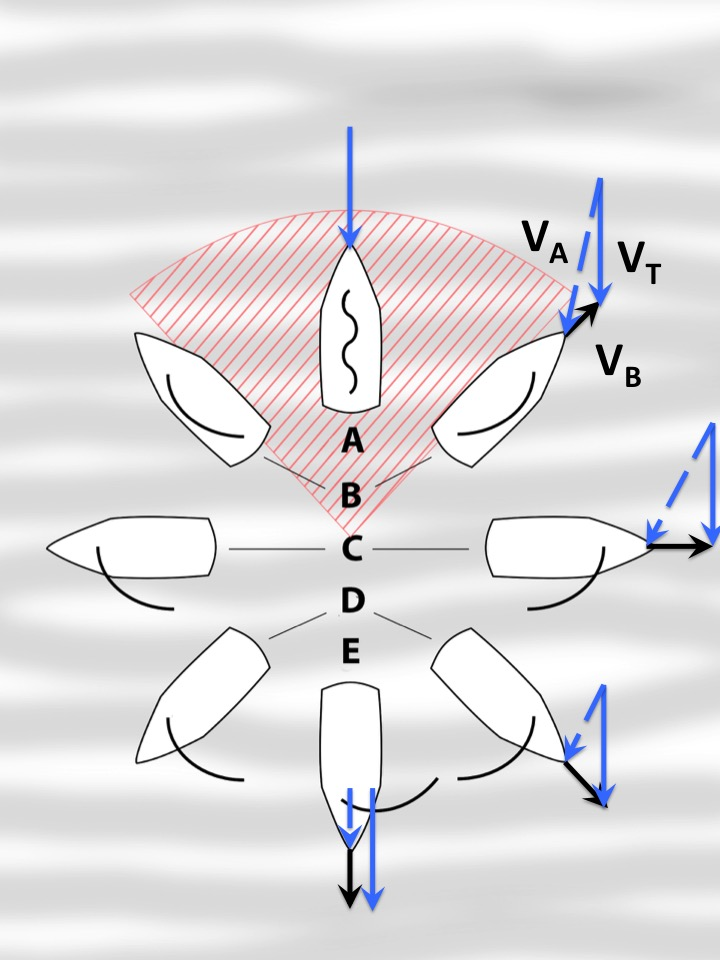
\includegraphics[width=0.6\textwidth]{Figures/Points_of_sail.jpg}
\caption{Points of sail.}
\label{points-sail}
\end{figure}
\begin{figure}[H]
\centering
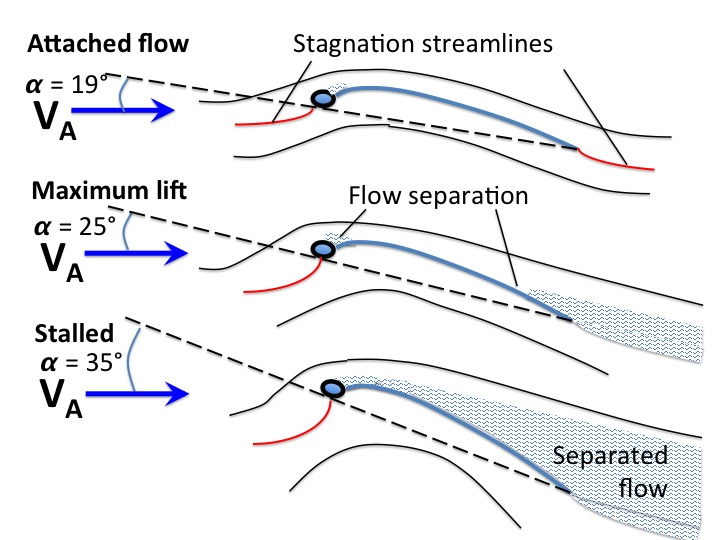
\includegraphics[width=0.5\textwidth]{Figures/max_lift.jpg}
\captionsource{Sail angles of attack.}{\url{https://en.wikipedia.org/wiki/Forces_on_sails}}
\label{max_liftl}
\end{figure}
\subsection{Velocity}
The main goal in sailing is to maximize the efficiency at which the forces on the sail translates into the velocity of the dinghy. A layman might expect the fastest velocity to be achieved when the dinghy is parallel to the true wind, this is however not true. The apparent wind, which is the wind experienced from the dingy perspective, is what propels the dingy. When sailing parallel to the wind the dinghies speed can never exceed the speed of the wind\cite{sail-force}. By sailing upwind close-hauled the apparent wind is increased as the dingy accelerates until the drag from the water exceeds the forward force created by the wind. To further increase the velocity, the dingy should not be heeling excessively. This is to prevent the centerboard from acting as a rudder and changing the bearing, introducing more drag from the stern rudder when compensating for the bearing changes. As mentioned earlier the centerboard helps to counteract heeling but also the sailor can prevent this by leaning out of the boat (hiking), to alter the center of mass for the dinghy. As a last resort the sailor must perform reefing to reduce the area of the sail to lower the center of effort from the sails.


\section{Product Application}
\label{sec:application}
\lipsum[9]

\subsection{Navigation and Tracking}
\chapterauthor{Sjölund, Johannes (Theolin, Henrik)}
\lipsum[10]

\subsection{Speed optimization}
\chapterauthor{Sjölund, Johannes (Theolin, Henrik)}
\lipsum[11]


\section{Hardware Design}

\clearpage
\section{Sensors}
\chapterauthor{Lundberg, Josef (no one)}

Since all kinds of sailboats main feature is to move completely analogue without the need of fuel or electricity, the use and optimization of surrounding forces are of foremost importance. Measuring this will provide the sailor with all the information needed to optimize the way they move and control their dinghy.

To get any kind of measurements of the dinghy, sensors are needed. As of now there are sensors measuring a wide array of items. This section will talk about these sensors; what they measure, where they were purchased, the requirements on the sensor, their features, drawbacks and also how they were implemented.
Since the sensors have to work in this particular system prototypes are made around the sensors to acquire the data.
Designs are made with the \gls{cad} software Fusion 360\cite{cad}. The models are manufactured using a 3D printer for fast and easy development.

\subsection{Force sensors}
The function of the daggerboard is to compensate for the force that the wind is pushing on the sail which also helps to hold the dingy level in the water. The goal is to have a system that can measure the forces that pushes on the daggerboard by the water it goes through. By measuring the side forces on the board, a rough estimation of the exerted force on the sail can be made. 


\subsubsection{The implementation}
After some different solutions was suggested the final sensor and measurement method was chosen as the most prominent and clean approach. This is shown in \autoref{Press_sens_impl}.
Important to know is that every solution is mandatory to be waterproof and sealed properly from the harsh environment that this system has as its home turf. 
With this implementation the daggerboard itself will not be disassembled or modified in any way. 
Solutions that required the sensors to be mounted on the outside or in parts that would be in danger if a crash might occur was scratched.  
Other solutions are, either way, more difficult to apply and mount or more complex.  

\begin{figure}[H]
\begin{center}
	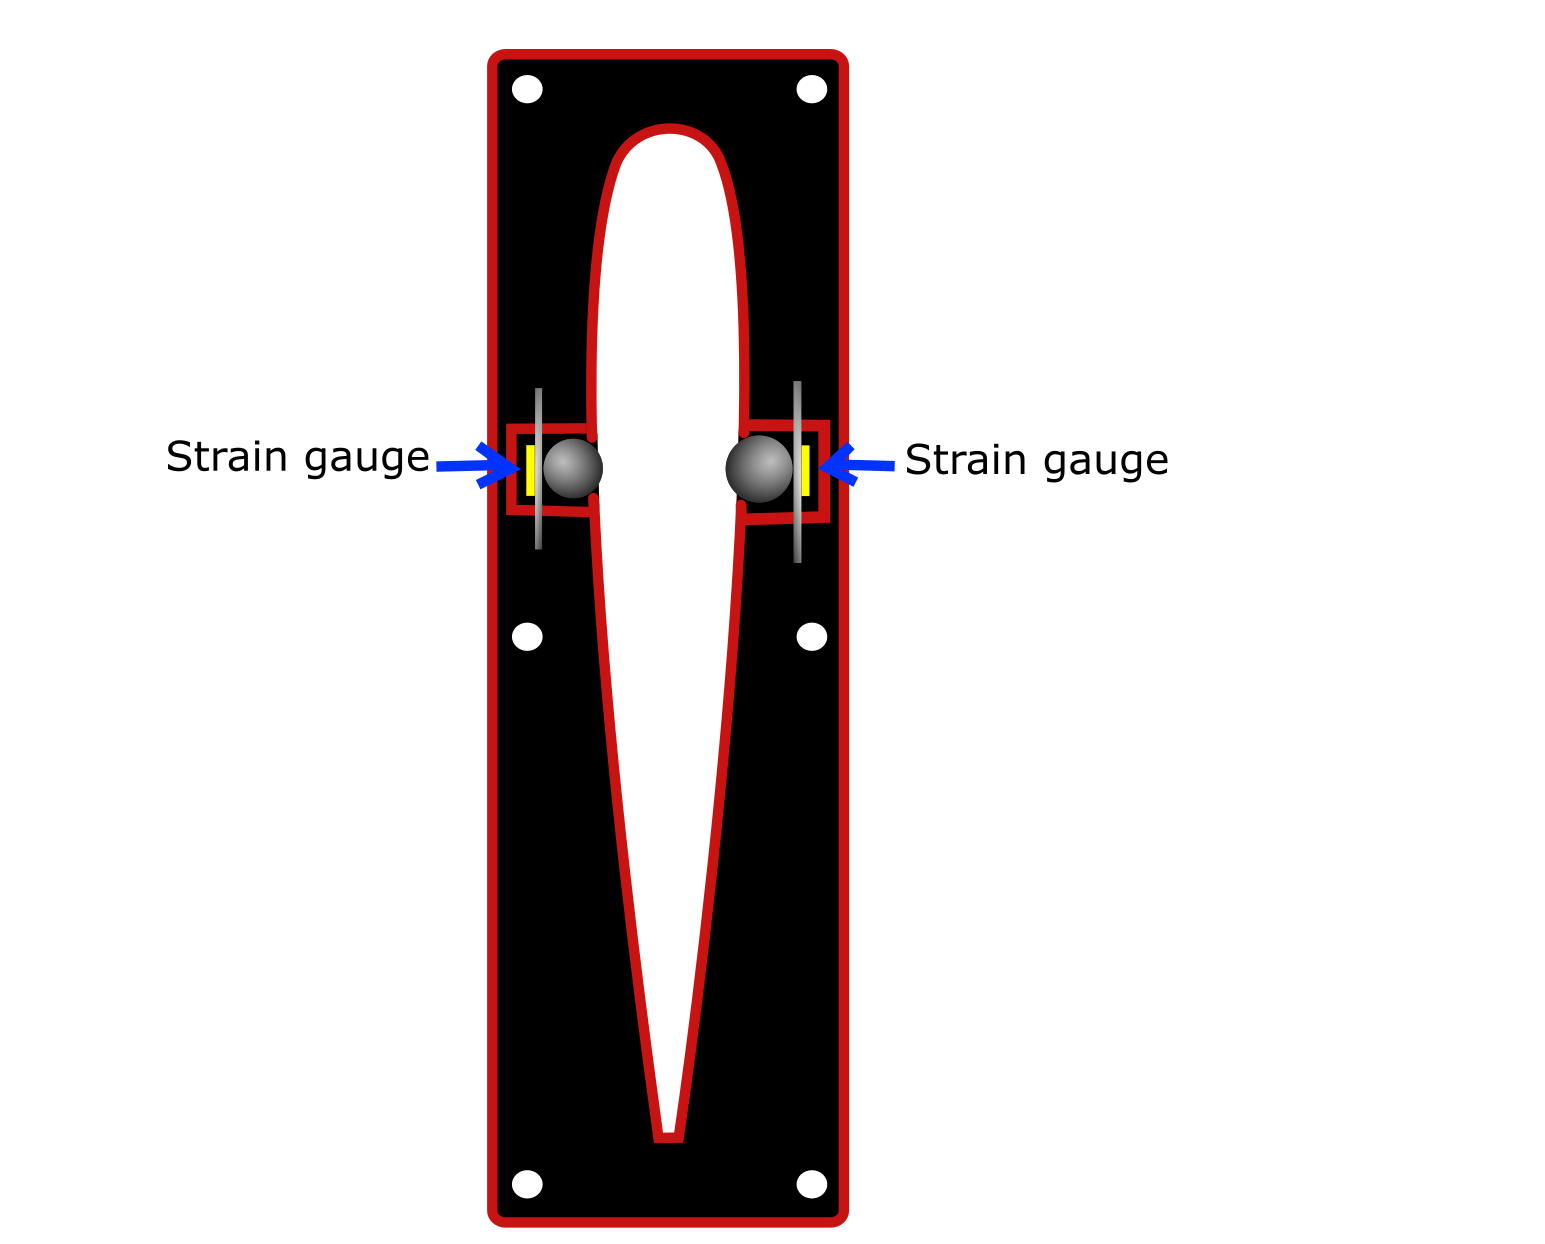
\includegraphics[width = 10cm]{Figures/Prototyp_1.png}
	\caption{Function of first prototype.}
	\label{Press_sens_impl}
\end{center}
\end{figure}

\subsubsection{The prototype}
To implement the gauges, a prototype is designed to show how the measurements will be made. The prototype is a bit bigger than the intended solution for this project but it is good to see how it would be constructed. The function is easy to understand. The board goes on the outside and can easily slide up and down past this steel bead. The bead itself is kept inside a small space where it can move in and out.

A model of the pressure sensor was created in order to clearly show the function of this sensor and to help the thought process involved in the improving of this design.

\begin{figure}[H]
\begin{center}
	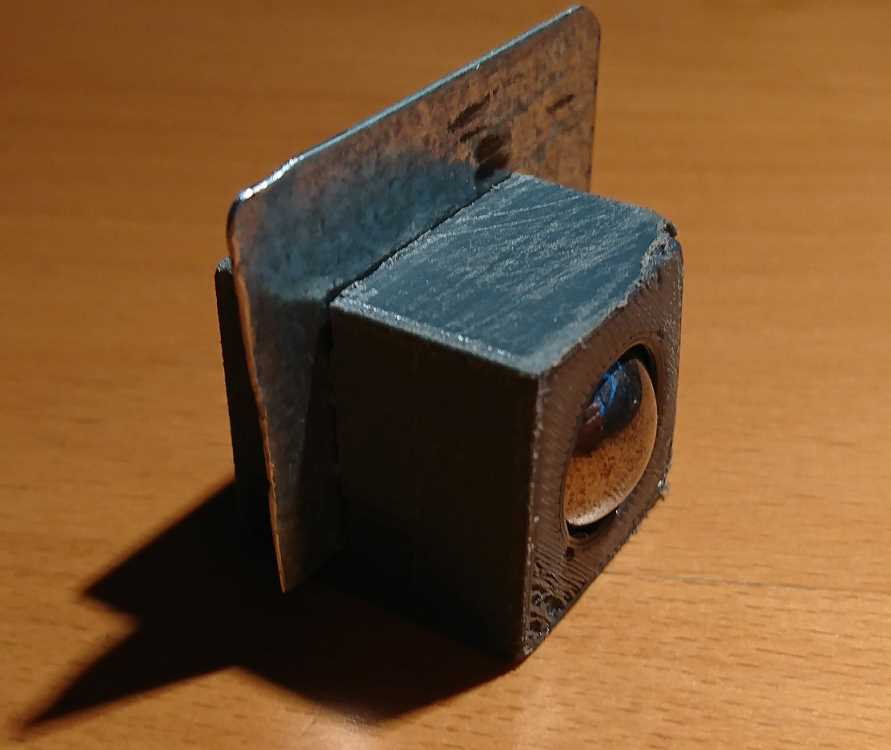
\includegraphics[width = 45\textwidth]{Figures/Press_sens_prot_1.jpg}
	\caption{First prototype of a force sensor.}
	\label{Press_sens_prot_1}
\end{center}
\end{figure}

The force is measured at the back where there will be a plate. The deflection of this plate which will be the origin to the strain will be measured through strain gauges. 
The gauge itself will measure a small difference in resistance. This small difference is going to be difficult to measure without any amplifying circuit connected. With a such small signal the system might have issues with noise. Another problem is the signal might drift, and therefore make different measurements as the circuit is running. And finally, with the measured values getting amplified with a big amount the resulting signal may be off by a large amount. 

A better solution is to make some research into load cells, which is a sensor which also utilizes strain gauges to measuring forces. The difference is that the gauges are already implemented in the sensor. The difference in this prototype is instead of having a metal plate, it can be built with a piece of plastic or rubber which can deform so the force is distributed directly to the sensor. By implementing this sensor, a lot of time was saved in troubleshooting. And by having a sensor unit, the modified mounting plate will be easier to produce. 
 
\begin{figure}[H]
\begin{center}
	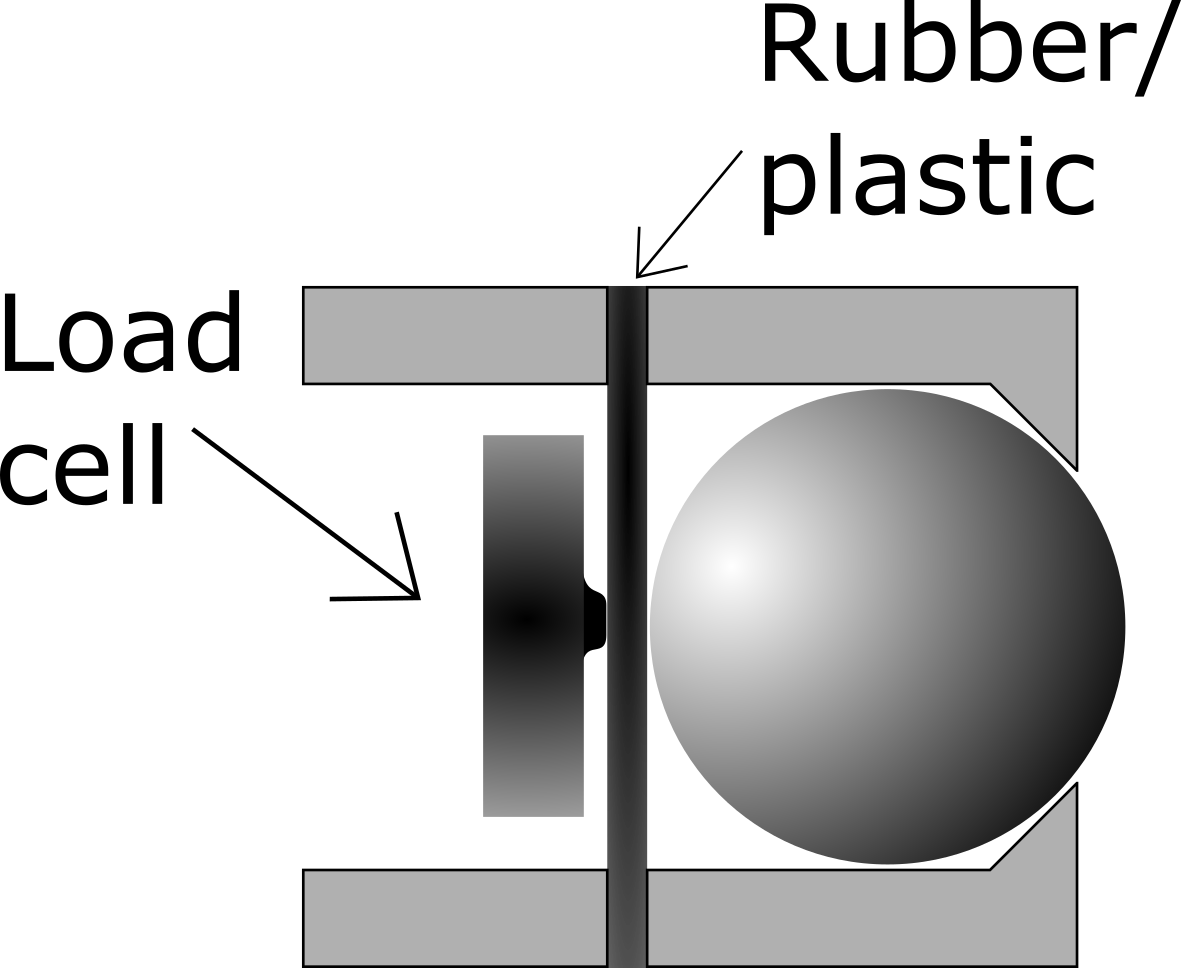
\includegraphics[width = 10cm]{Figures/Press_sens_func_2.png}
	\caption{Function of second prototype.}
	\label{Press_sens_prot_2}
\end{center}
\end{figure}


\subsubsection{Sensor}
The force from the board onto the mounting plate will be a considerable amount. The actual force is something that is not known for sure. The initial assumption was that a load cell with a $90.75$ kg force range should be enough. If the sensor will be maxed out, the cell its rated for a $150\%$ overload without causing some damage to the sensor.  

The chosen sensor for this application is this part, the compression load cell called FX1901\cite{load_cell}.  
From the datasheet, the voltage readings of this part could be calculated. The maximum voltage difference is calculated to be around $180mV$. 

\begin{figure}[H]
\begin{center}
	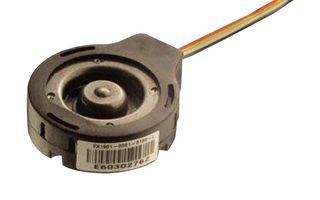
\includegraphics[width = 10cm]{Figures/Load_cell.png}
	\caption{Load cell, FX1901}
	\label{Load_cell}
\end{center}
\end{figure}


\subsection{Amplifier}
With a such small signal, an amplifier is needed to get some desired measurements. A good measurement signal to the \gls{mcu} should be in the order of in between$0–3.3$ volts. Since the maximum value from the load cell is $180mV$ an signal of $3.3$ volts is achieved by an amplification gain of around $20$.  
A suitable amplifier needs to be chosen from this implementation. Inspiration is taken from The University of Chicago\cite{UoC} in an experiment where they use this exact load cell together with an instrumental amplifier called INA125. This amplifier is somewhat more complicated and has some more features that other amplifiers.  

In the same family of instrument amplifiers, a model called INA126\cite{ina_126} is selected as a less complicated and more power efficient solution.  
This amplifier has a smaller power draw due to some simpler functions and lesser precision. But for this application it is sufficient.  
The implementation is easy and the gain can easily be determined by connection a resistor Rg between two pins on the amplifier. 

\begin{figure}[H]
\begin{center}
	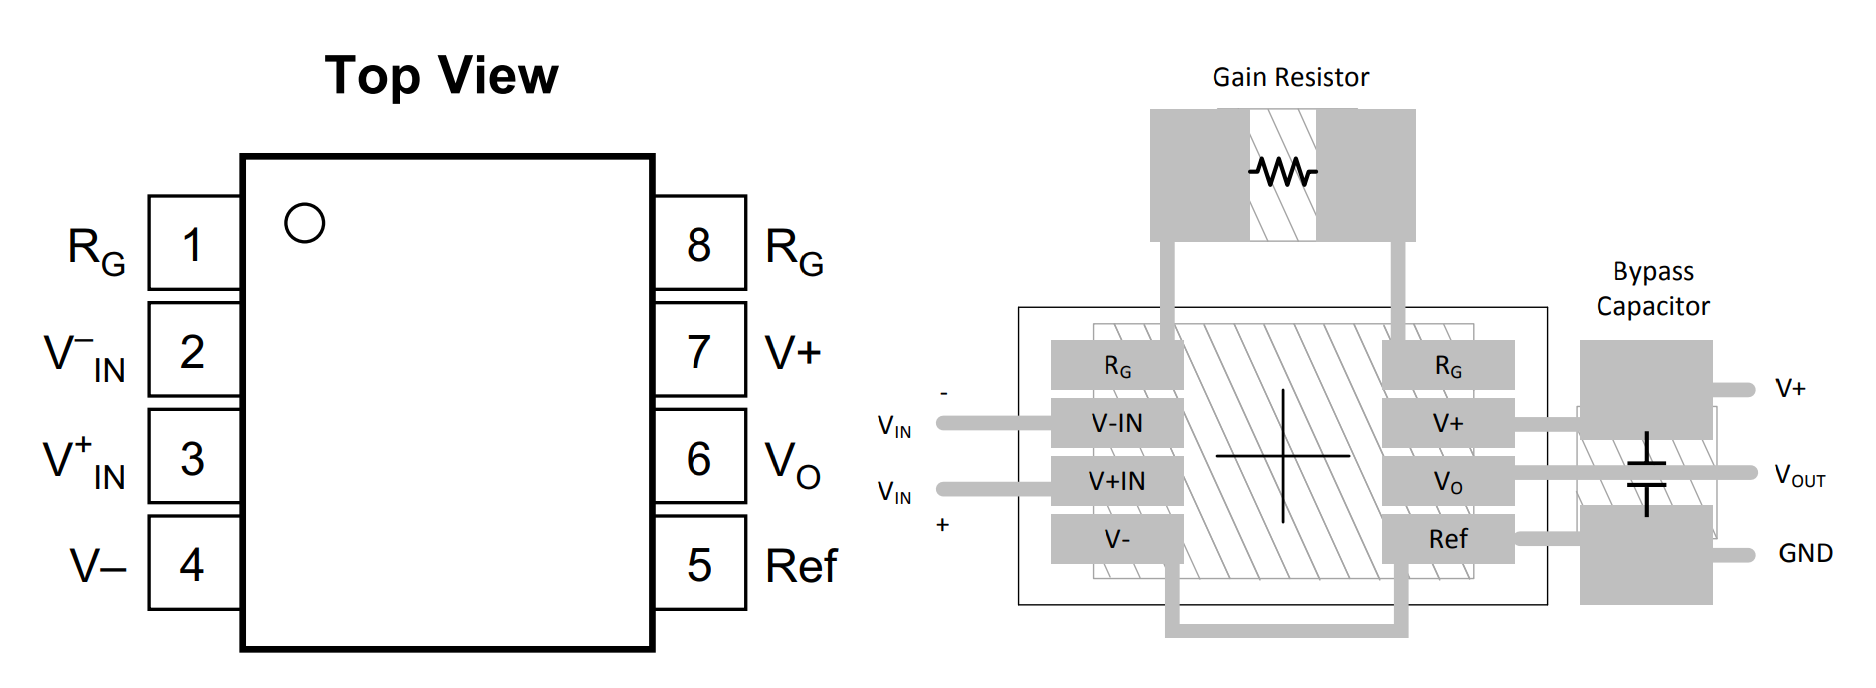
\includegraphics[width = 10cm]{Figures/INA126_pinout.png}
	\caption{Amplifier for the load cell signal.}
	\label{INA126}
\end{center}
\end{figure}

The gain on this piece is easily calculated with following function.  

\begin{equation}%add a \label{labelname} to refer to this equation.
\textrm{Gain} = 5 + \frac{80~\textrm{k}\Omega}{R_G}
\end{equation}

In order to adjust the gain of the amplifier the resistor $R_G$ is set to a fixed resistor in series with a potentiometer.


\subsection{Height of centerboard sensor}
The height of the daggerboard is a crucial measurement in dinghy sailing. The daggerboard not only gives the dinghy a corresponding force to the sail, the board can also be a danger if you sail in running wind. One of the best implementations of a height sensor would be the use of a linear wire distance sensor. This sensor measures how far a wire is pulled, which gives a very accurate measurement. This solution can be totally watertight and concealed in the main centerplate. Other solutions can be to use some type of light sensor. 

\subsubsection{Sensors}
%The sensor fulfilling our requirements of both functionality and size is the following, NAME, see fig. (\ref{FIGURELABEL}). It is ..

A suitable product has been found, which is very accurate and reliable, the Micro epsilon mk30\cite{micro-epsilon-mk30}.

It's physical volume in small enough with a size of 3x5cm. As the product have some tight space constraints this can probably fit inside the case. This particular sensor is in the range of 2000kr. If no other solution works as intended this might be considered again.
The main issues might be that the height of centerboard: % That the height of the centerboard what?
One of the best implementations of a height sensor would be the use of a linear wire distance sensor. This particular sensor measures how far a wire is pulled, which gives a very accurate measurement. This solution can be completely watertight and concealed in the main centerboard.  

\begin{figure}[H]% As mentioned before, H -> tb, Refer to all figures used, use width only to /restrict/ size.
\begin{center}
	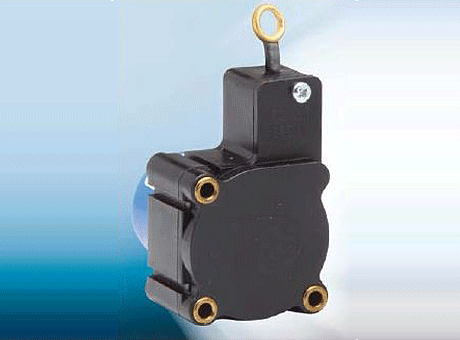
\includegraphics[width = 10cm]{Figures/microepsilon_mk30.png}
	\caption{Linear draw wire sensor, Micro epsilon MK30.}
	\label{Draw_sensor}
\end{center}
\end{figure}

Light sensors have also been considered. This is implemented with the use of a plate placed on top of the dagger-board and with the light being sent up to this panel, the height can be calculated. First, we looked into some \gls{ir}-sensors. They will send the signal in a widespread which will make the distance measurement troublesome as this signal has just a small plate to bounce off.

With the use of a \gls{lidar} system, we can point our light signal at an exact spot and then get an exact measurement of the height.  
Many of the \gls{lidar} systems found was both too large and expensive to be implemented in this project.
A new product called "micro-lidar" can be used, as it is both have a small form factor and is easy to implement.
The chosen circuit is VL53L0X from Adafruit\cite{micro_lidar}. 

\begin{figure}[H]
	\centering
	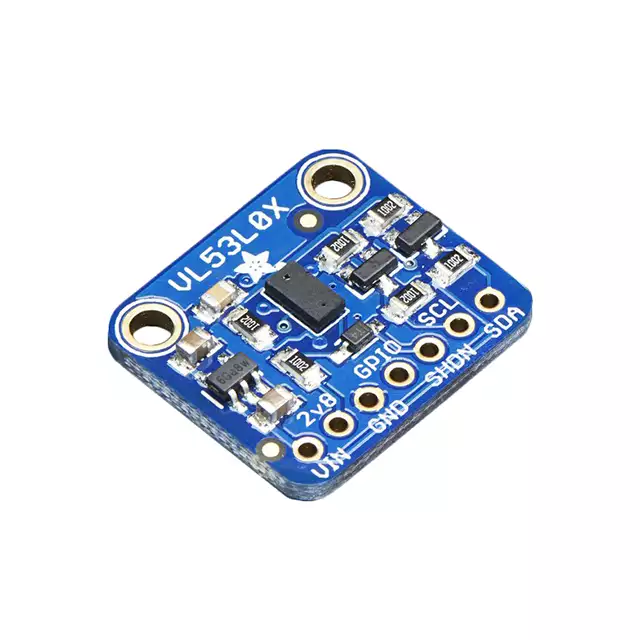
\includegraphics[width = 10cm]{Figures/Adafruit_height_sensor.png}
	\caption{Time of flight, $\mu$\gls{lidar}, distance sensor Adafruit VL53L0X.}
	\label{micro_lidar}
\end{figure}

It can measure heights up one meters with great accuracy and communicates with \gls{i2c}.

By the fact that the sensor must be waterproof the signal has to go through a medium. The medium can be some type of plastic or even glass.   

All the information about this sensor when used with a cover widow can be found in the specific datasheet: “VL53L0X ranging module cover window guidelines” \cite{Tof_cover}. The maximum thickness of the cover window and the air gap between the sensor and the window is 2 mm. That’s the parameters that need to be considered. The cover window can be some type of plastic or glass. To reflect the signal a detection plate is constructed and fastened to the top of the daggerboard. This plate is level with the sensor and has a white underside for best performance of the sensor. 

\begin{figure}[H]
	\centering
	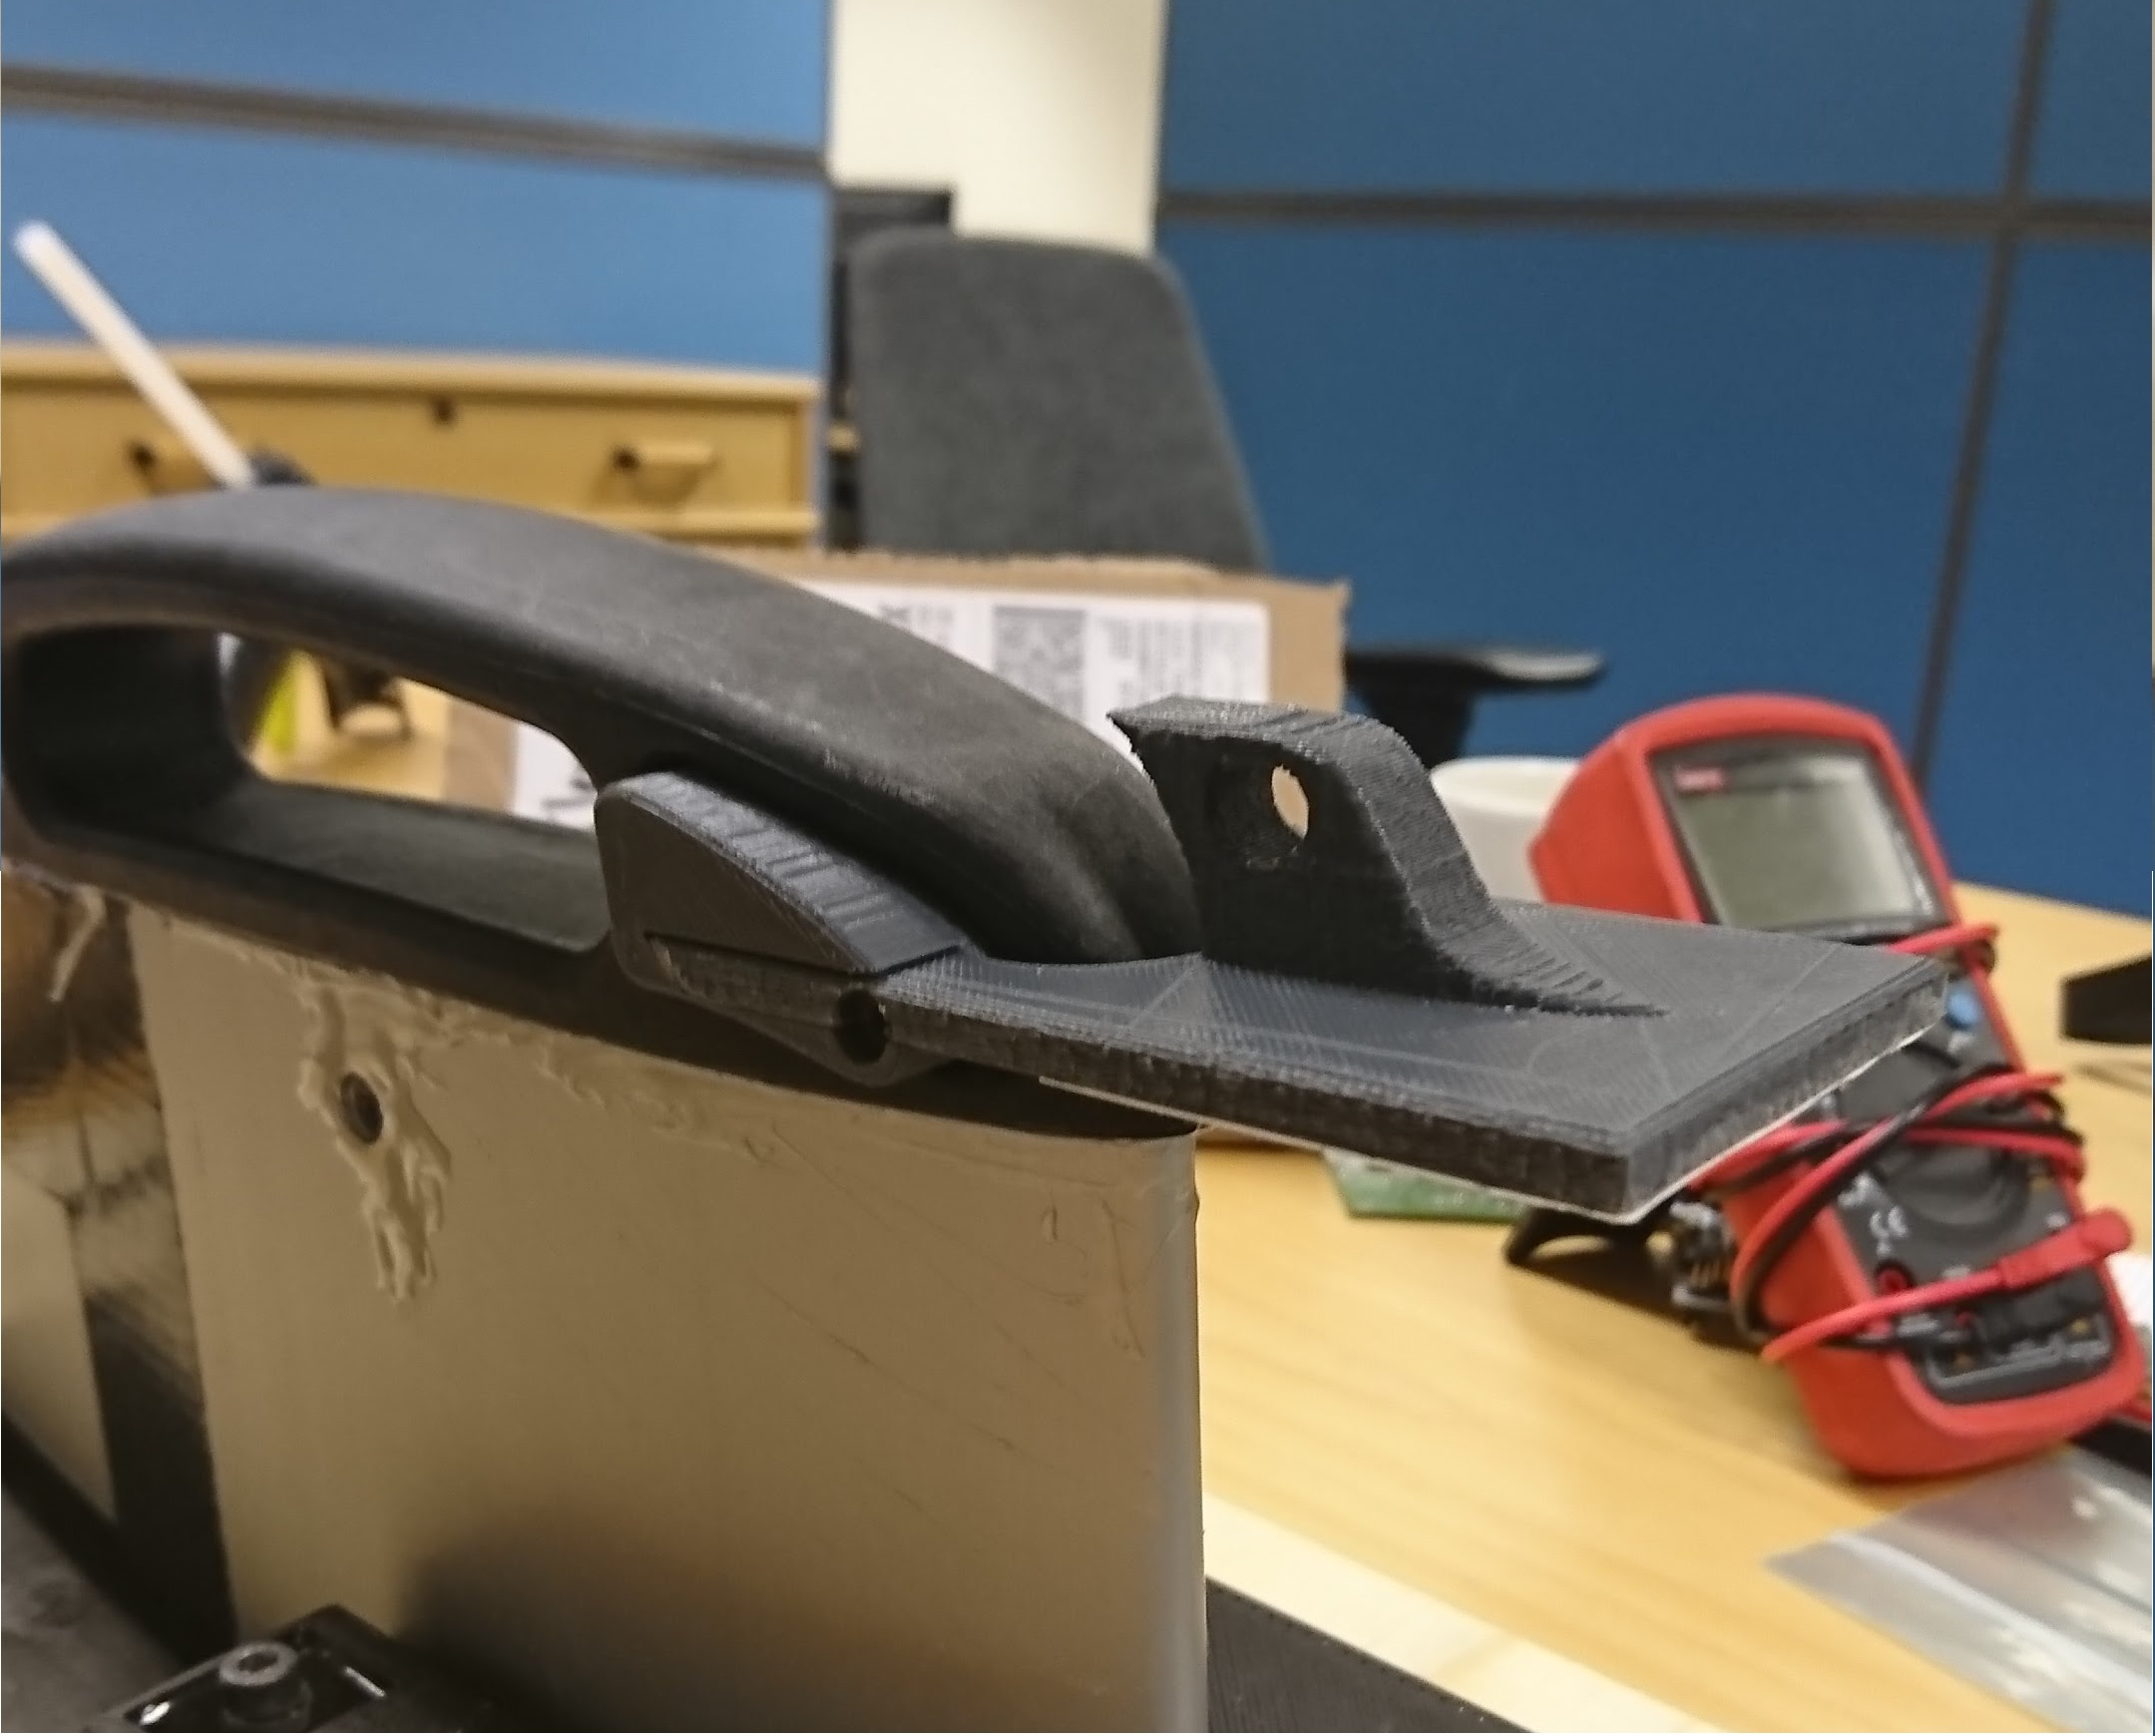
\includegraphics[width = 10cm]{Figures/height_measure.jpg}
	\caption{Height measurement model.}
	\label{height_measure}
\end{figure}


\subsubsection{Results}

The sensor works very well in the open air and can detect heights up to 1.5 meters with great accuracy. It also works well when used behind a thin plastic cover. With a 1mm thin plastic cover the maximum heigt measurement is decresed to about one meter. In the case the sensor is mounted behind a thin epoxy window witch was to thick at the beginning but was sanded down to a sutible thickness. The final window were then polished to a crystal clear finish for the best measurements. The measurement is heavily dependent on the the finish of the window, if there is small inperfections on the window such as scratch the sensor can't take measurements.

As there will always be water around and on the center plate the light that is sent might get directed "wrong" if there are only some small water droplets in between the sensor and the panel that we want to reflect our light on.  

This system can definitively be improved in the future with either a completely different measurement system or with a better implementation of the window cover. The window cover probably would work better if the cover was molded in a convex form, which could lead off the water droplets formed on the window surface. This in cooperation with a surface finish that repels water, such as a hydrophobic coating would be a great solution. 




\clearpage
\section{Software Design}
\chapterauthor{Sjölund, Johannes (no one)}
The software has been divided into two parts, the firmware for the ARM MCU with associated sensors, and an Android application which can display sensor data. These two parts utilize a Bluetooth connection to communicate their current states. For example, when the IMU calculates a new orientation, this data should be processed by the firmware, and the resulting calculations sent to the Android application over Bluetooth to be displayed to the user.

\subsection{ARM firmware}

\begin{figure}[H]
\centering
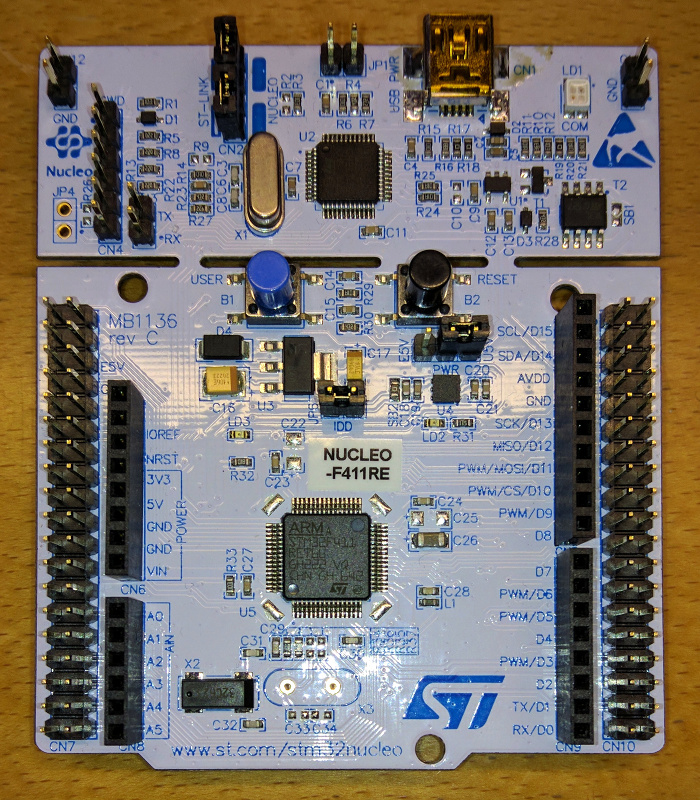
\includegraphics[width=0.6\textwidth]{Figures/stm32nucleo.jpg}
\caption{}
\label{nucleo-board}
\end{figure}

For rapid prototyping and firmware development purposes, the NUCLEO-F411RE development board seen in figure \ref{nucleo-board} was used. This board contains break-out pins for the ARM Cortex-M microcontroller STM32F411RE, a UART to USB bridging circuit and general purpose LEDs and buttons. It is compatible with various Arudino shields as well as expansion boards developed by ST.

In order to speed up firmware development, the STM32CubeMX \cite{stm32cubemx} initialization code generator was used to set up a basic working system. This application, developed by ST, can generate C language code for setting up MCU clocks, peripherals, interrupts and similar. It is controlled by a graphical interface for setting MCU options and controlling the previously mentioned code generation.

The main challenge in working with this type of code generation is integrating it with external software libraries directly not built for it. If the library interferes with generated code by overriding settings and register values, the software may enter an undefined state and stop working. Care therefor had to be taken to only use the parts of the libraries which did not interfere. Frequent testing of any newly added functionality had to be done in order to find interfering parts.

Two libraries produced by ST were used, one for the Bluetooth module, and one for the IMU.

\subsubsection{Bluetooth}
\label{bluetooth}

\begin{figure}[H]
\centering
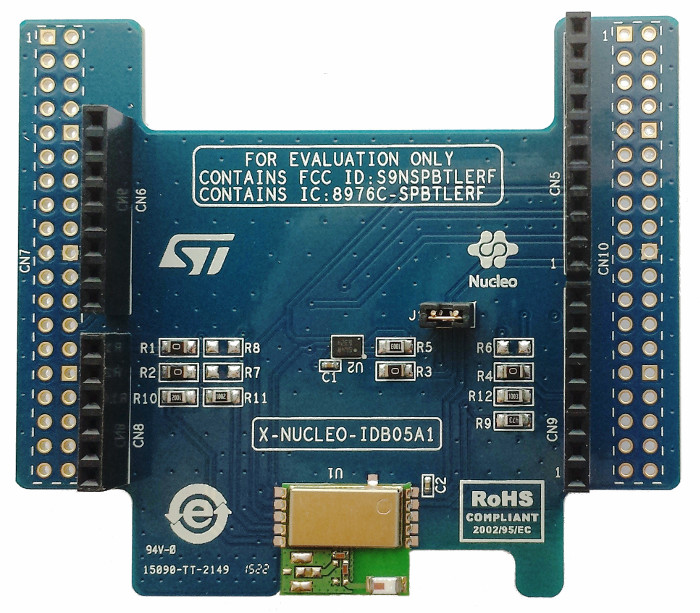
\includegraphics[width=0.6\textwidth]{Figures/x-nucleo-idb05a1.jpg}
\caption{}
\label{bt-eval-board}
\end{figure}

For prototyping, the Bluetooth evaluation board X-NUCLEO-IDB05A1 \cite{x-nucleo-idb05a1} seen in figure \ref{bt-eval-board} was used, which could be stacked on top of the Nucleo board. The pins on the evaluation board connected it to and SPI port on the MCU.

To avoid having to implement the Bluetooth stack from scratch, the firmware package called X-CUBE-BLE1 \cite{x-cube-ble1} developed by ST was used. It consisted of several parts -- MCU and Bluetooth evaluation board device definitions such as named pins and ports, functions for manipulating them, a Bluetooth GATT server implementation, as well as several demo applications showing usage examples. Additionally an Android demo application for displaying sensor data from Bluetooth was available from the Google Play platform, called BlueNRG \cite{bluenrg-app}. The library code was integrated into the code generated by STM32CubeMX, added as an external library and statically linked.

While ST included example code for communicating with the Bluetooth module over SPI through interrupt based DMA transfer, this code was quite difficult to get working. Instead it was decided that blocking SPI communication were to be used, since this was much simpler to get working. The reasoning was that since the module supported a baud rate of up to 10 Mbit/s, this would be fast enough to cause miminal interference with other parts of the firmware code.

\begin{figure}[H]
\centering
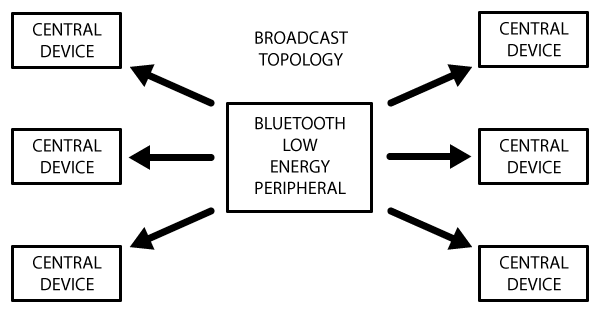
\includegraphics[width=0.6\textwidth]{Figures/bt_gap.png}
\caption{Bluetooth GAP topology.}
\label{bt-gap}
\end{figure}

\begin{figure}[H]
\centering
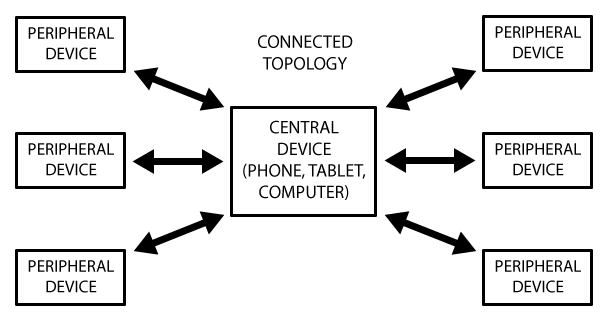
\includegraphics[width=0.6\textwidth]{Figures/bt_gatt.png}
\caption{Bluetooth GATT topology.}
\label{bt-gatt}
\end{figure}

As mentioned previously, the library implemented the Bluetooth GATT protocol. This protocol supports bidirectional communication from a single central device, in this case an Android cell phone, to several peripheral devices, such as the embedded system in this project. The library also supported the Bluetooth GAP protocol, which is a unidirectional communication protocol allowing one peripheral device to broadcast to multiple central devices. Figures \ref{bt-gatt} and \ref{bt-gap} illustrates the topological differences between these protocols.

For this project, the GATT protocol was chosen. The reasoning was that enabling the Android app to send commands to the embedded system could be useful for controlling functionality. This meant that only a single phone could be connected to the system at any time, as opposed to the GAP protocol, which would allow multiple phones to listen to the Bluetooth broadcasts. Since the embedded system is designed to be used on a small dinghy with space for a maximum of two people, this seemed like a reasonable trade-off. If the system was to be used on a larger sail boat, the GAP protocol might be more useful, since it would allow multiple passengers to listen to broadcasted sensor data.

\begin{figure}[H]
\centering
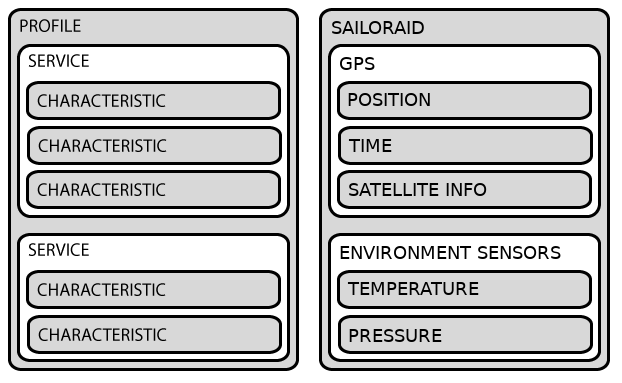
\includegraphics[width=0.6\textwidth]{Figures/bt_gatt_profile.png}
\caption{Bluetooth GATT transaction profile with usage example.}
\label{bt-gatt-profile}
\end{figure}

The GATT protocol performs transactions by nested structures called Profiles, Services and Characteristics. An example of this structure can be seen in figure \ref{bt-gatt-profile}. These structures were already implemented in the X-CUBE-BLE1 and updated by simple function calls. When new sensor data was received from e.g. the GPS or IMU devices, these functions were called at regular intervals which pushed the data to the Android app. Each profile were given a unique identifier which allowed the app to recognize which type of data was received.

\subsubsection{IMU}

\begin{figure}[H]
\centering
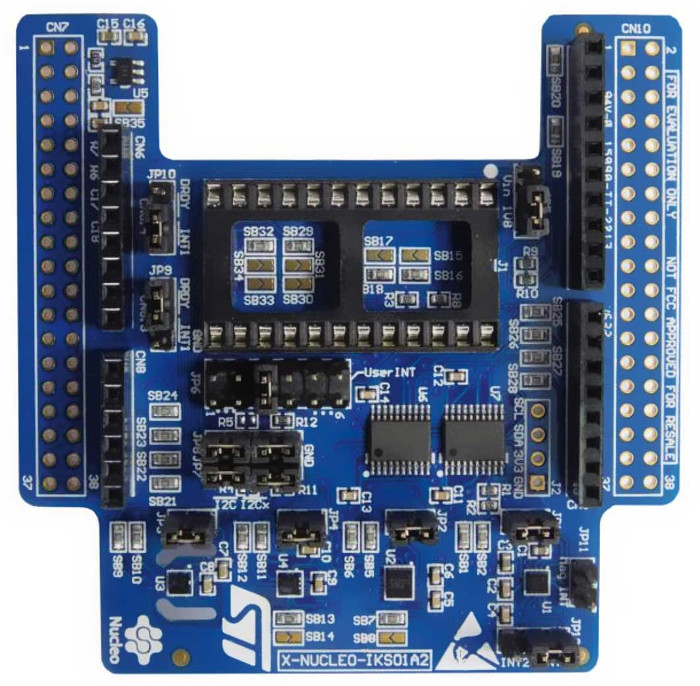
\includegraphics[width=0.6\textwidth]{Figures/x-nucleo-iks01a2.jpg}
\caption{}
\label{imu-eval-board}
\end{figure}

In order to measure the various time dependent spatial features such as orientation, acceleration and velocity, an IMU device was used. More specifically, the X-NUCLEO-IKS01A2 \cite{x-nucleo-iks01a2} evaluation board (figure \ref{imu-eval-board}) developed by ST was chosen for rapid prototyping purposes. This board included the LSM6DSL 3D accelerometer/gyroscope, the LSM303AGR 3D accelerometer/magnetometer, the HTS221 humidity and temperature sensor as well as the LPS22HB pressure sensor.

To interface the firmware with the board, the X-CUBE-MEMS1 \cite{x-cube-mems1} library developed by ST was used. This library implemented the I$^2$C communication protocol used by the previously mentioned IMU devices in the form of simple function calls, which saved a lot of development time. It was quite simple to integrate with the code generation from STM32CubeMX, only a few source definitions had to be modified. Like with the Bluetooth library (section \ref{bluetooth}) blocking communication was chosen to simplify the code, even though the MCU supported interrupt based DMA transfers. The I$^2$C operated in fast mode at 400 kHz which was thought to cause minimal interference with the rest of the system in blocking transfer mode.

An important use case for the IMU was to determine the current orientation of the dinghy. To accomplish this, a type of sensor fusion algorithm called Madgwick AHRS (section \ref{madgwick}) was used.

\subsubsection{Madgwick AHRS}
\label{madgwick}
Madgwick AHRS \cite{madgwick} is a type of sensor fusion algorithm which calculates the current orientation in space from three dimensional vectors of acceleration, angular velocity and magnetic field strength. It was developed in 2010 by Sebastian O.H. Madgwick as a more performant alternative to the Kalman filter approach. It basically integrates the angular velocity from the gyroscope, while using the accelerometer and magnetometer to create a reference to the horizontal plane. Earth’s magnetic poles provides a horizontal vector which lies on the plane, while the gravitational acceleration is the plane’s normal vector. This then used by the algorithm to compensate for drift in gyro integration. The algorithm stores orientation in quaternions (rotation vectors with four elements), but can convert it to Euler angles, which can be more easily used.

The mathematical background of this algorithm is quite complicated and outside the scope of this report, see the official report \cite{madgwick-report} for more details.

\subsubsection{USB UART}
Since this project involved analyzing sensor data for developing sensor fusion algorithms, for example combining GPS and accelerometer for accurate positioning (section \ref{ekf}) and measuring water wave properties, it was important to be able to log data at a reasonably high frequency. To this end, a hardware UART-over-USB chip was used, the ST-LINK/V2-1 on the Nucleo board, and FTDI FT232R on the custom project board.

\todo{MATLAB serial read}

\subsubsection{GPS}

\subsubsection{Range sensor}

\subsection{Android application}
\chapterauthor{Theolin, Henrik (Axelsson, Oskar)}
The main reason for this project is to give a sailor qualitative feedback and help in clearing the mind of the techniques required to achieve a smooth sail experience so that the sailor can focus on the joy of sailing.
A crucial part is to display the data in a manner that is easy to interpret and provide the help that the skipper needs.

To further increase the flexibility of the design, several different user layouts are implemented, that the user can switch between while running the application. This was determined to be a good way of increasing the chances that the user would find a preferable layout.

It was also determined that not only visual representation was enough, since the sailor needs to be in constant motion to counteract the forces applied on the ship by the wind and currents. This will make watching a screen to retrieve information somewhat difficult.
Other ways of representing data were implemented using text-to-speech where the sailor will get important information by sound as well as text
 Vibration is also implemented with different vibration sequences depending on different states of the ship.


\subsubsection{Software design}
A \gls{uml}\cite{uml} model of the system, see \autoref{android-uml}, was developed for an overview of the system implementation. The android system uses activities\cite{activity} to display content to the device screen. These activities have a life-cycle (\autoref{android-activity}) that determine how data is accessed and displayed. What should be understood is that the application starts in a main activity, and switching to another activity is done by sending an intent that spawns as a child activity.
While the application is in the child activity the main activity is paused but the state is stored and when switching back from the child all data from the previous state is being accessed.
When the user returns from the child activity,  that activity is destroyed and all data is erased.
Sending data between activities is done using intents, to send an intent to a child activity is done by adding a bundle with a data object along with the intent to spawn the child activity.
Sending data back to the child activity is done by calling the method ``\emph{startActivityForResult}'', this allows the child to send a data packet as a result back to the parent. 
\begin{figure}[H]%Can this be put in the Appendix? It is very large and detailed.
\centering
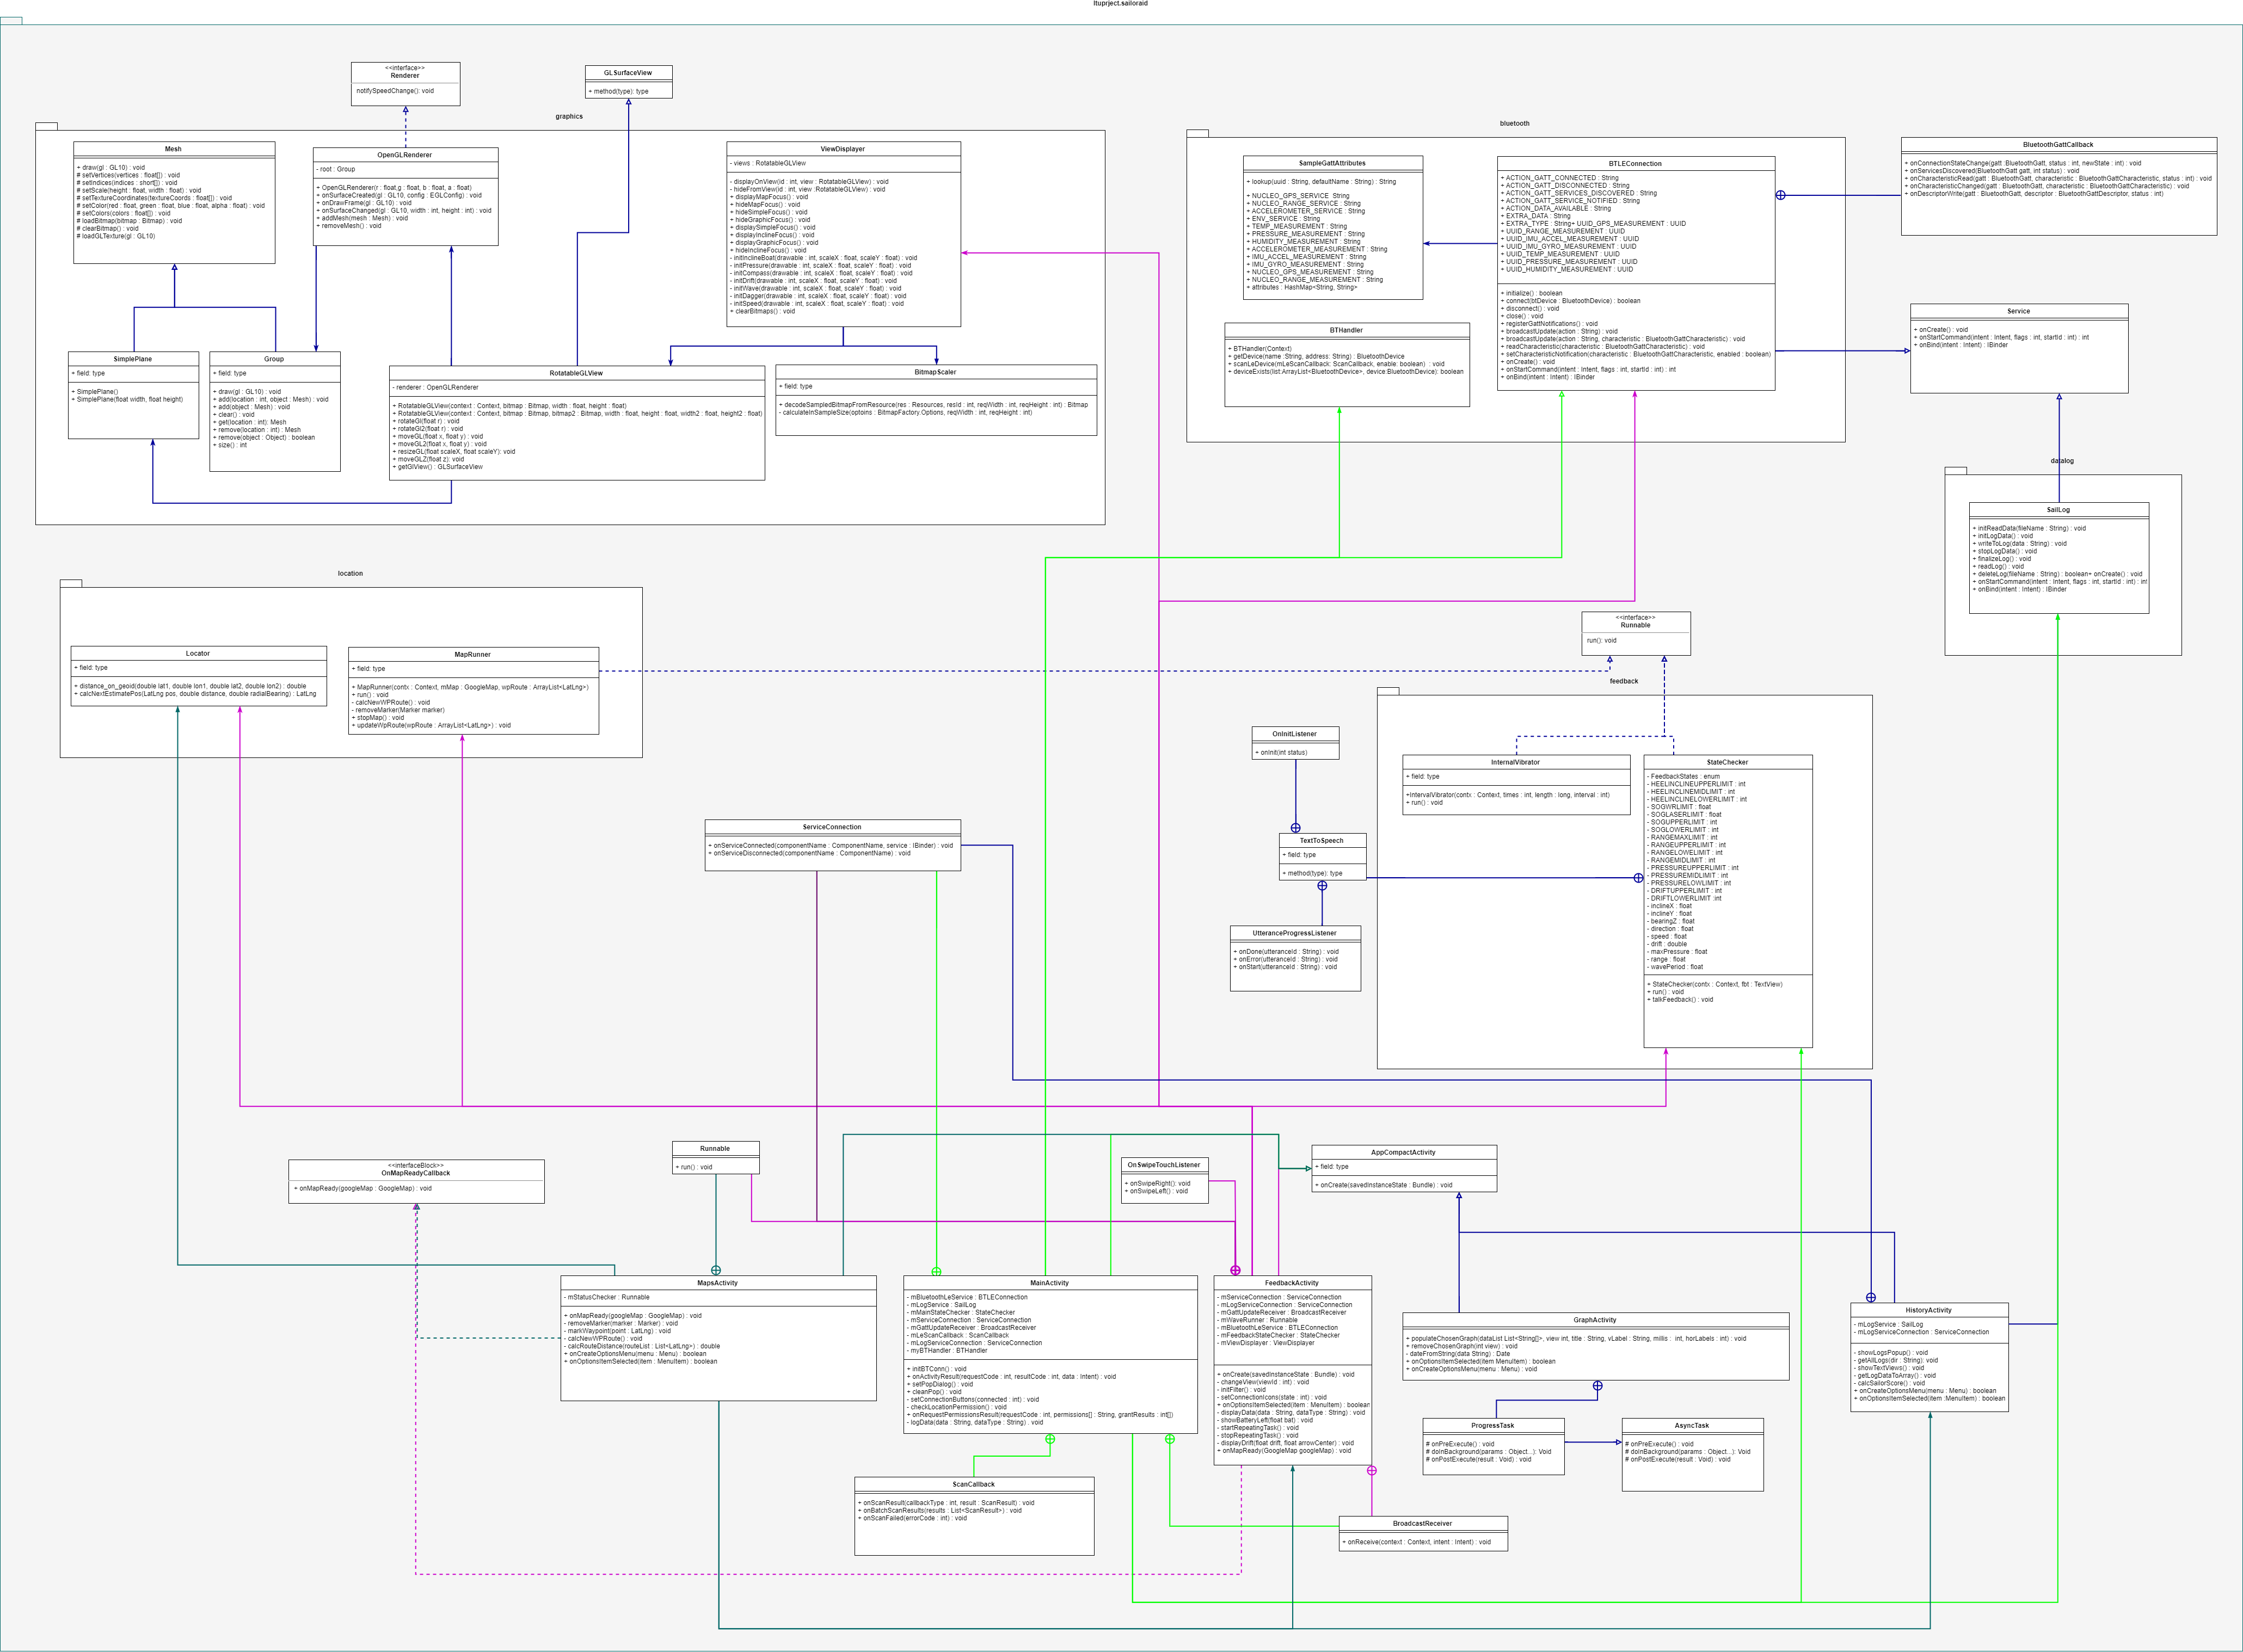
\includegraphics[width=\textwidth]{Figures/uml.png}
\caption{\gls{uml} model.}
\label{android-uml}
\end{figure}
\begin{figure}[H]
\centering
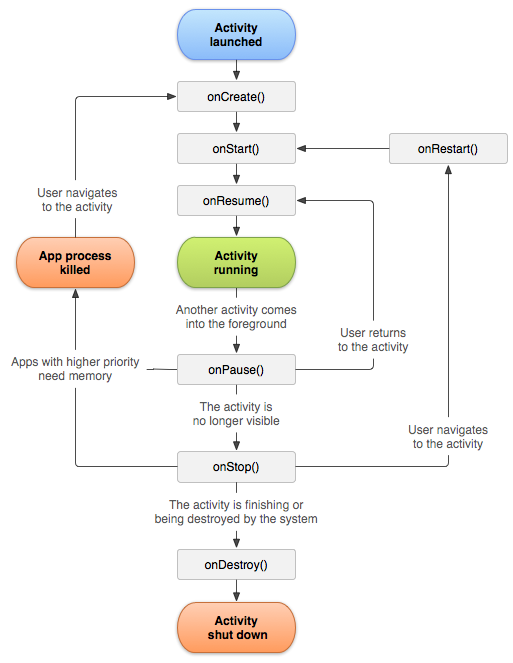
\includegraphics[width=0.8\textwidth]{Figures/activity_lifecycle.png}
\captionsource{Activity lifecycle.}{ Author}
\label{android-activity}
\end{figure}

The Bluetooth connection and data logging class is implemented as a services\cite{android-service}. A service can be started by an activity and continue running until it is explicitly called to stop. This allows several activities to share resources and perform long-running operations in the background. The lifecycle of a service is seen in \autoref{android-service}.
\begin{figure}[H]
\centering
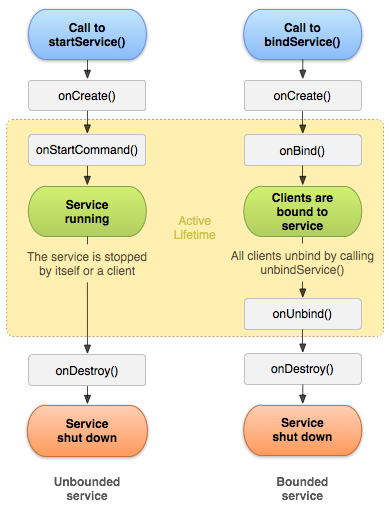
\includegraphics[width=0.8\textwidth]{Figures/service_lifecycle.png}
\captionsource{Service lifecycle.}{Author}
\label{android-service}
\end{figure}

\subsubsection{Feedback}
For the feedback states in the application, there are some approximations, and simplifications made for easier implementation. As explained in \autoref{sec:physics}, the chapter about Physics of sailing, there are certain parameters that can be evaluated in different states of the dinghy. An extensive approximation is that there is no water movement in the implementations. The states implemented are
\begin{labeling}{alligator}
\item [Clear] - The dinghy holds good velocity and not heeling or drifting and with a good amount of pressure on the dagger-board
\item [Drift] - The dinghy is drifting perpendicular to the bearing while the dagger-board is in an upper position
\item [Heel] - The dinghy has high heel angle
\item [Reefing] - The dinghy has high heel angle and the pressure on the dagger-board is high
\item [Wrspeed] - The dinghys speed is above $65.45~\textrm{kn}$
\item [Lrspeed] - The dinghys speed is above $16.8~\textrm{kn}$
\item [Hike] - The dinghy has more then moderate heel angle and the pressure on the dagger-board is between medium and high
\item [Keelhaul] - The dinghy has an above moderate heel angle and the dagger-board is not in the lowest position
\item [Runninghigh] - The dinghy is sailing directly windwards with dagger-board high and low heel angle.
\item [Runninglow] - The dinghy is sailing directly windwards with dagger-board high and mid heel angle.
\item [Landcrab] - The dinghys speed is low.
\end{labeling}
Given these states, appropriate feedback can then be provided to the user. For handling states, a class called \emph{StateChecker} was implemented. This stores sensor values and check against limits defined at an interval that is also defined in the class. Depending on these states this class also determines what feedback that should be given.

\subsubsection{Visual Feedback}
It was determined that the visual feedback provided to the user was to include very little text information and would consist mainly of figures that changed position based on sensor data to give a good representation of what was going on with the dinghy. Because of different personal preferences, the ability to switch between different layouts is implemented. This is done by a simple swipe on the screen to toggle the view to the next layout. All layouts consists of a subset of views from the complete set including
\begin{labeling}{alligator}
\item [\ref{feedback-incline} \textbf{Incline}]  displays a ships relative incline against and artificial horizon.
\item [\ref{feedback-pressure} \textbf{Pressure}] moves a pin along a colored bar to represent high of low pressure applied on the dagger-board.
\item [\ref{feedback-compass} \textbf{Bearing}] rotates a compass to show the ship relative bearing against true north.
\item [\ref{feedback-map} \textbf{Map}] displays current location of the ship.
\item [\ref{feedback-height} \textbf{Speed}] displays a speedometer from a classical Swedish vehicle\cite{volvo} with a movable bar representing speed over ground.
\item [\ref{feedback-drift} \textbf{Drift}] is represented with a colored bar containing two arrows that moves to the relative drift direction to show the sailor if the ship was holding its set navigational reference.
\item [\ref{feedback-text} \textbf{Feedback}] a text that changes values based on the current state of the boat.
\item [\ref{feedback-sog} \textbf{Height}] of the dagger-board is represented with a visual dagger-board moving up and down along a graphical ruler.
\item [\ref{feedback-wave} \textbf{Wave frequency}] displays a wave moving towards a ship at a speed representing different period of the waves.
\end{labeling}

\begin{figure}[H] 
 	\centering
	\begin{minipage}[c]{0.6\textwidth}
	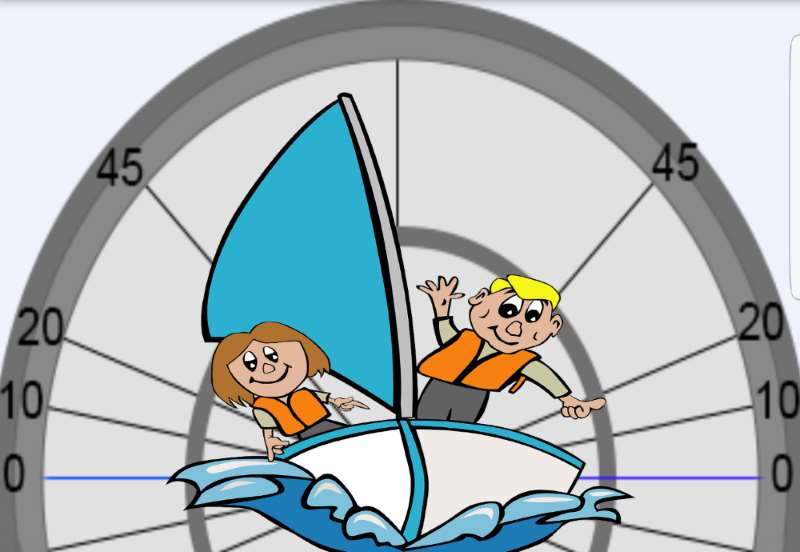
\includegraphics[width=\textwidth]{Figures/incline.jpg}
	\captionsource{Incline feedback view}{\url{https://pixabay.com/en/sailboat-children-playing-kid-girl-23801/}}
	\label{feedback-incline}
	\end{minipage}
	~
	\begin{minipage}[c]{.3\textwidth}
	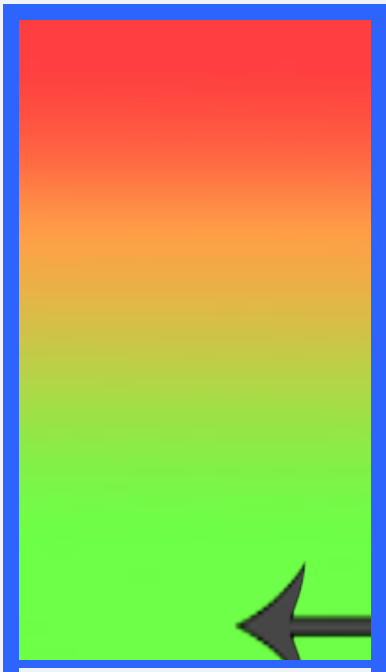
\includegraphics[width=\textwidth]{Figures/pressure.png}
	\captionsource{Pressure feedback view.}{Author}
	\label{feedback-pressure}
	\end{minipage}
\end{figure}
%
\begin{figure}[H]
	\centering
	\begin{minipage}[c]{0.55\textwidth}
	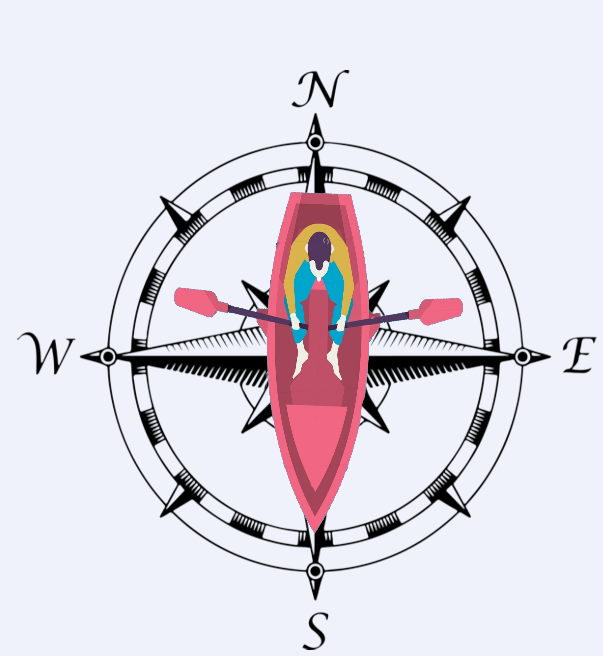
\includegraphics[width=\textwidth]{Figures/compass.png}
	\captionsource{Bearing feedback view.}{\url{http://www.pngall.com/compass-png}}
	\label{feedback-compass}
	\end{minipage}
	~
	\begin{minipage}[c]{0.35\textwidth}
	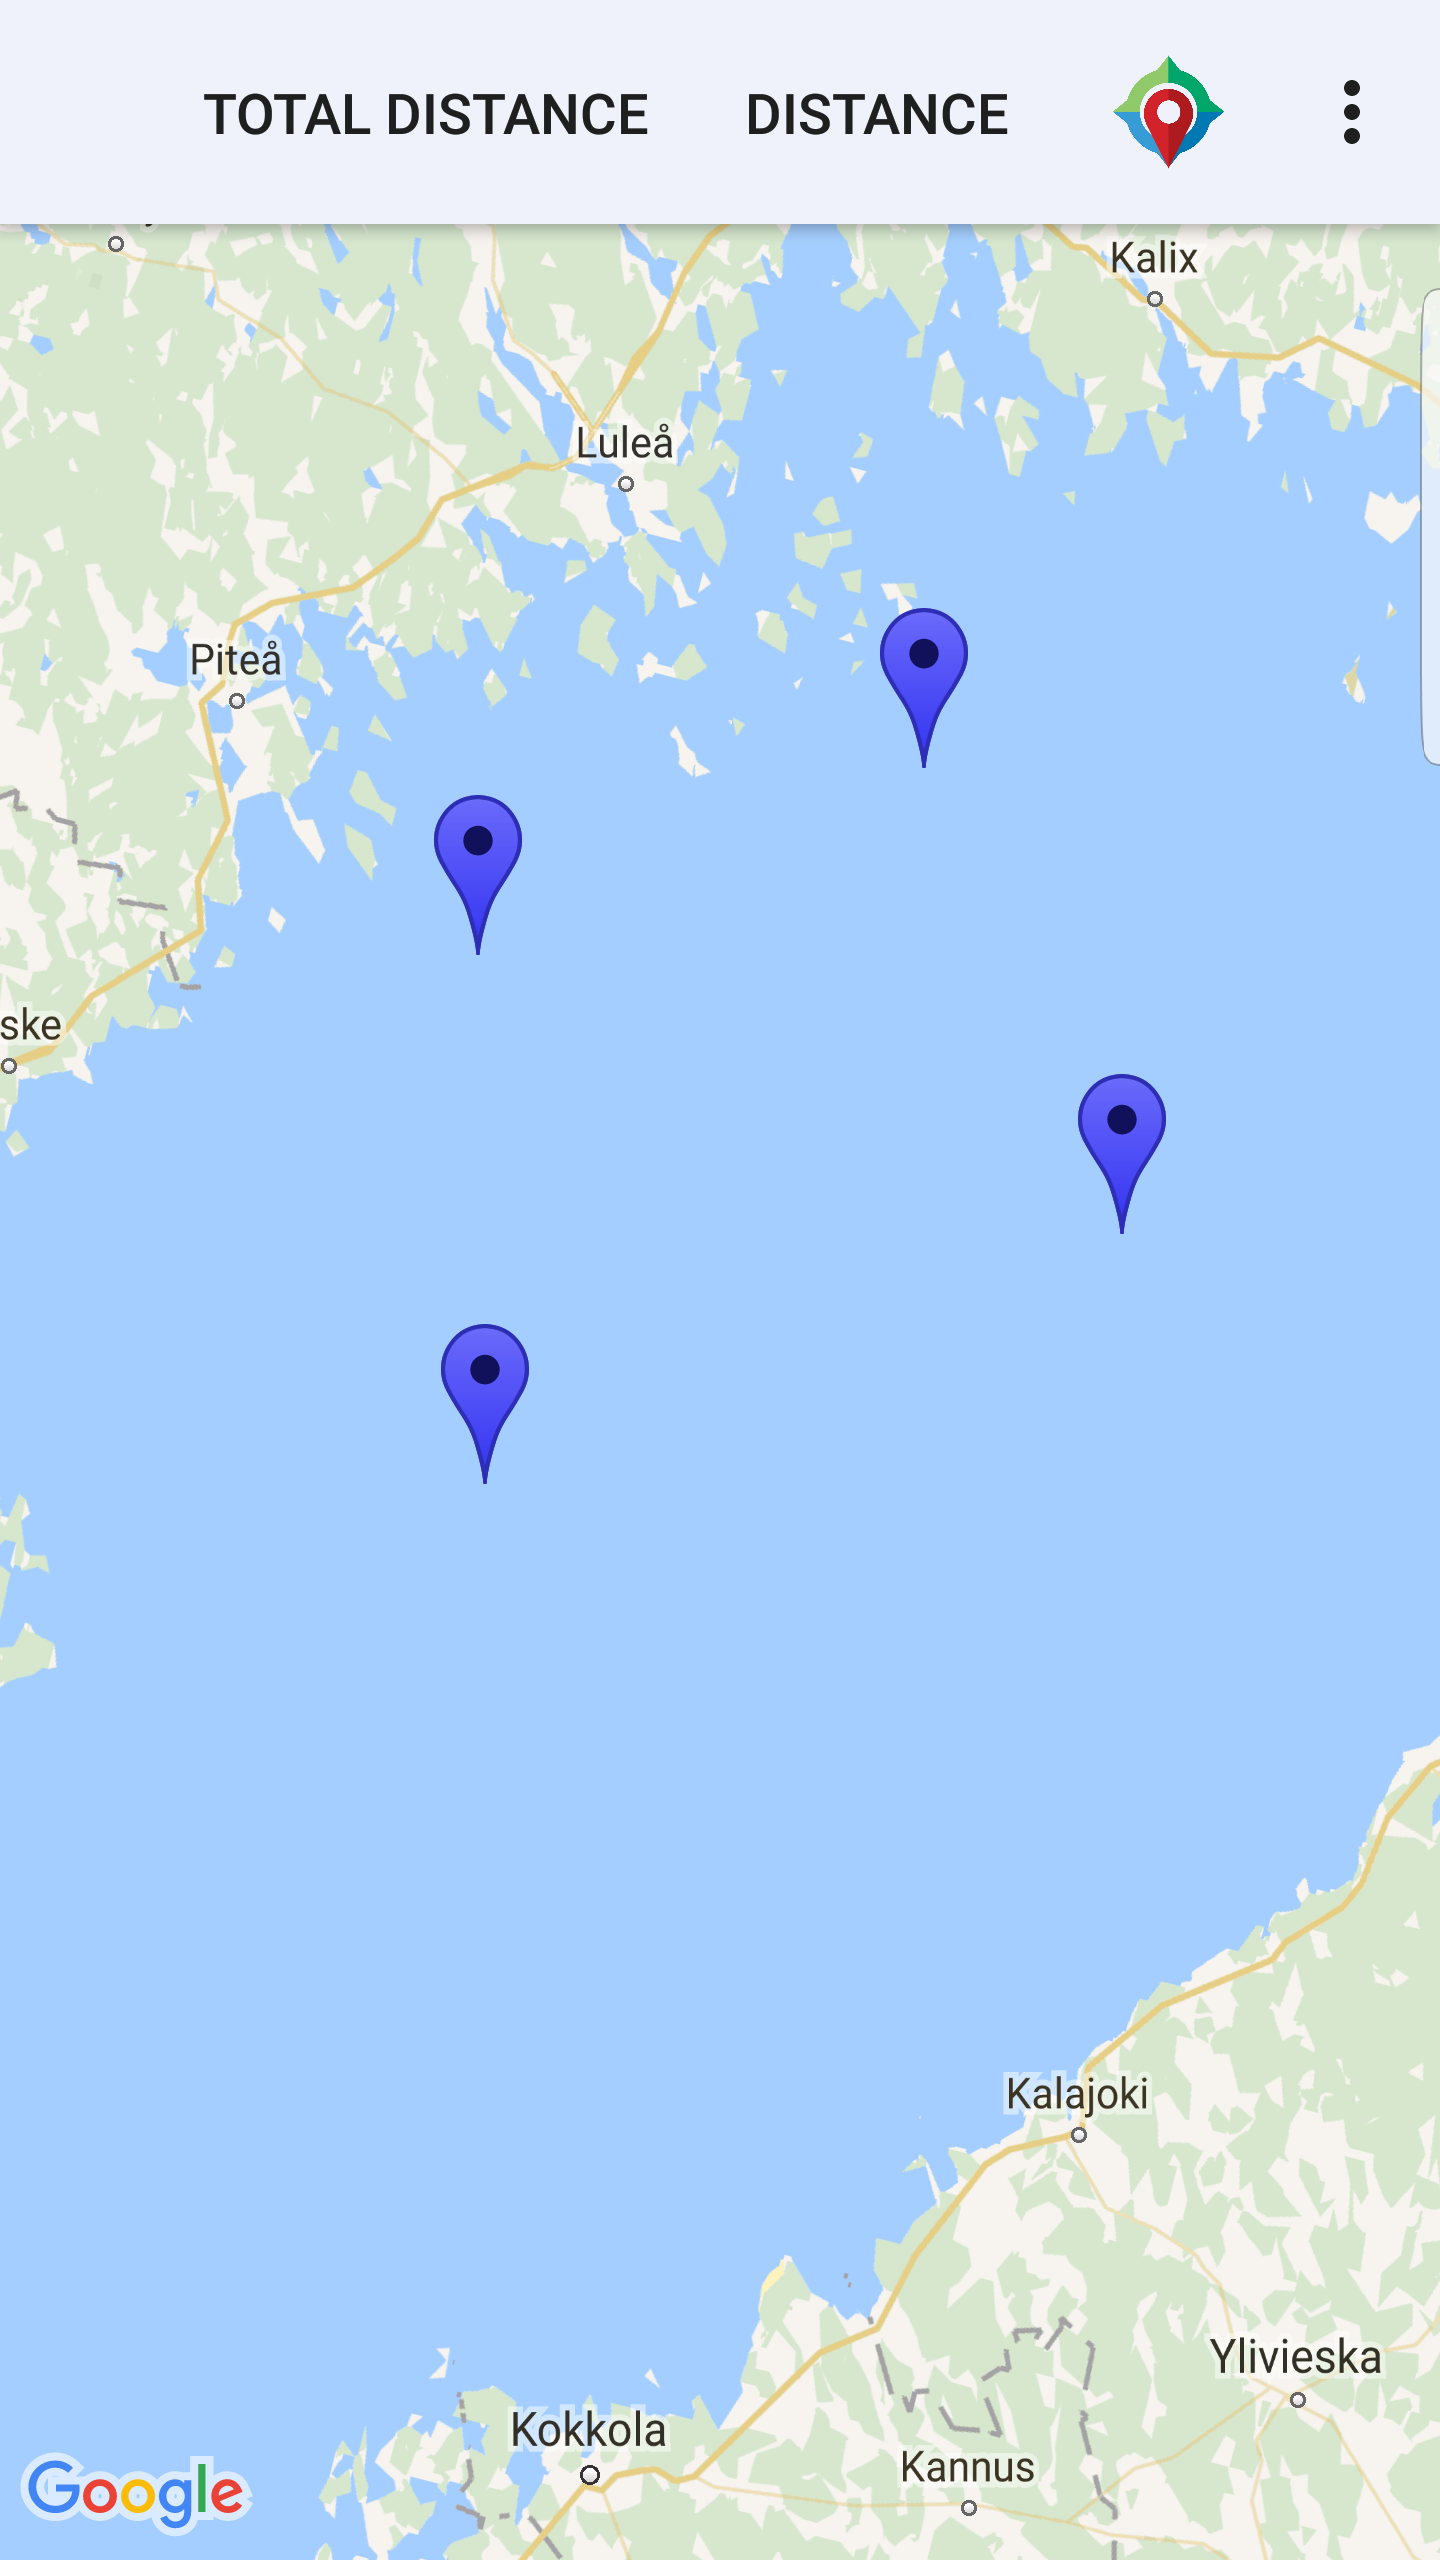
\includegraphics[width=\textwidth]{Figures/map.png}
	\captionsource{Map feedback view.}{Author}
	\label{feedback-map}
	\end{minipage}
\end{figure}
\begin{figure}[H]
	\centering
	\begin{minipage}[c]{0.35\textwidth}
	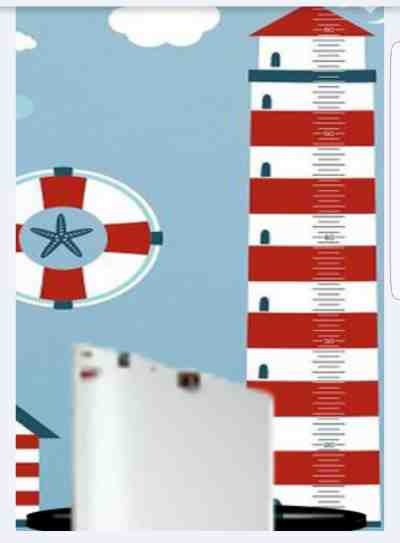
\includegraphics[width=\textwidth]{Figures/height.jpg}
	\captionsource{Dagger-board height view.}{\url{https://www.pinterest.se/pin/275212227218947579/}}
	\label{feedback-height}
	\end{minipage}
	~
	\begin{minipage}[c]{0.55\textwidth}
	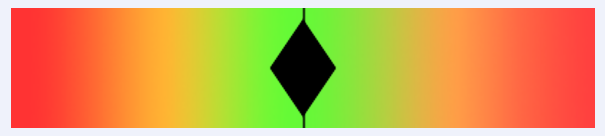
\includegraphics[width=\textwidth]{Figures/drift.png}
	\captionsource{Drift feedback view.}{Author}
	\label{feedback-drift}
	
	
\includegraphics[width=\textwidth]{Figures/text.png}
	\captionsource{Text feedback view.}{Author}
	\label{feedback-text}
	\end{minipage}
\end{figure}
\begin{figure}[H]
	\centering
	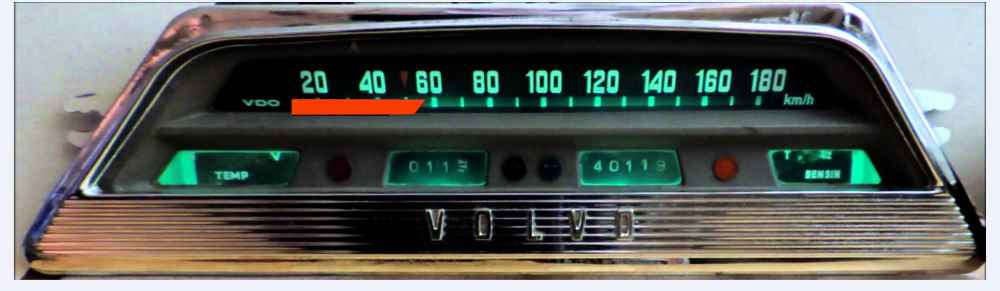
\includegraphics[width=0.8\textwidth]{Figures/sog.jpg}
	\captionsource{Speed over ground view.}{\url{https://youtu.be/k8M6ZHplbIU}}
	\label{feedback-sog}
\end{figure}
\begin{figure}[H]
	\centering
	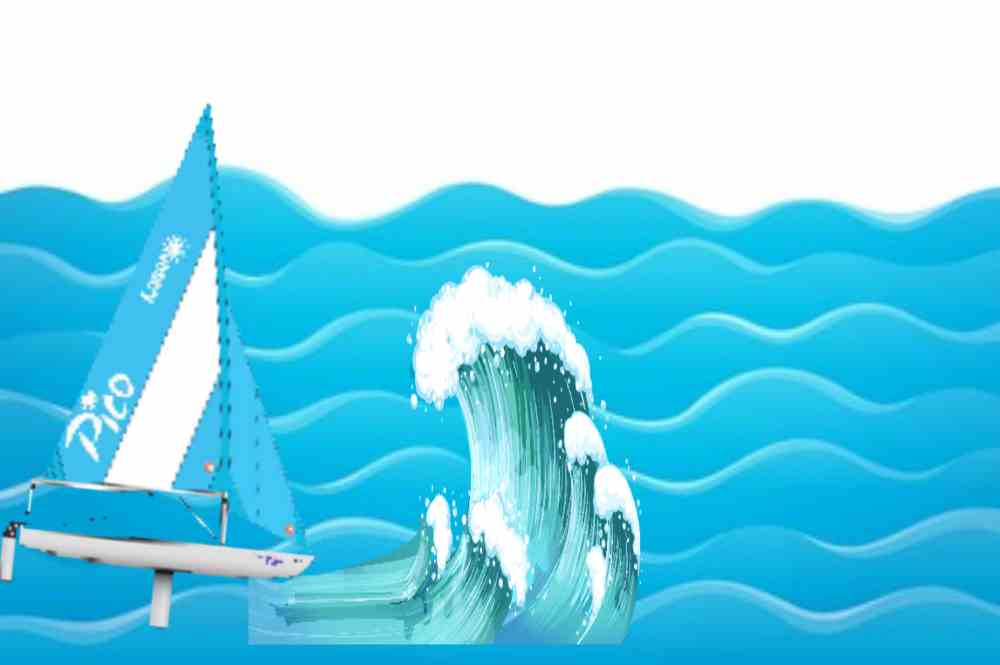
\includegraphics[width=0.8\textwidth]{Figures/wave.jpg}
	\captionsource{Wave period feedback view.}{Author, Stockfresh\#2886857, Dreamstime\#33314341, \url{http://shorelinesailboats.com/product/pico/}}
	\label{feedback-wave}
\end{figure}
The figures were chosen at a development stage and improvements can easily be made by adding different \gls{png}\cite{png} files in android studio. They are implemented as \emph{GLSurfaceView}\cite{gl} so that updating the figures is be done by calling a \emph{requestRender} function, this improves the performance of the application when only updates to the figures are done when new sensor readings are received. To make the figure fit the application the \emph{GLSurfaceView} is extended into a \emph{RotatableGLView} that has the wanted features for rotation and positioning. Using these figures four different layouts are developed to give multiple choices for the user and is seen in figure \ref{feedback-layouts}. Switching between these layouts a \emph{swipeTouchListener} is implemented which allows the user to swipe across the screen to change the layout. Changing view the figures needs to be redrawn onto a new view matching the current layout, this is handled in the \emph{ViewDisplayer} class that contained all \emph{RotatableGLViews}.

\begin{figure}[H]
\centering
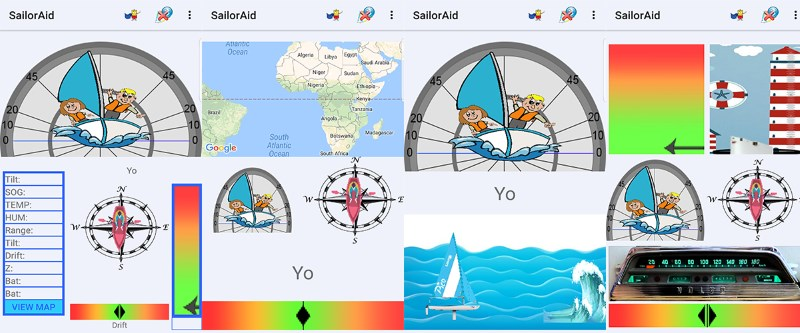
\includegraphics[width=0.9\textwidth]{Figures/layouts.jpg}
\captionsource{Different layouts}{Author}
\label{feedback-layouts}
\end{figure}

\subsubsection{Audio feedback}
Based on values from the sensors, different states are implemented and for each state, a text is read out to the user. The feedback is implemented such that the audio feedback would continue even if the device is put into sleep mode. Handling the text to speech feature a \emph{Text-to-Speech}\cite{texttospeech} class is implemented as an inner class in \emph{StateChecker}. To prevent the speech to be interrupted preemptively an \emph{UtteranceProgressListener}\cite{utter} is used. 

\subsubsection{Haptic feedback}
Based on the same states as the audio feedback vibration is also implemented. The frequency and length of the vibrations are implemented in such a way each state has a unique signature that can be recognized by the sailor after some practice with the system. Handling the interval an \emph{IntervalVibrator} is implemented and run by the \emph{StateChecker}.

\subsubsection{Log}
The ability to analyze the sailing trip was determined to be an important feature for the user, so a logging function is implemented so data can be stored in the device internal storage. This is handled by the \emph{SailLog} class and these files can be read or deleted at a later stage, by the user. Storing a log is implemented such that the sailor would need to start a logging session after Bluetooth connection has been established to the ship. After the log is started it creates a file on the device internal storage and writes sensor data to the file at the same frequency as the data is transmitted by the system. While logging is active the device would continue to store information even if the device is put in sleep mode so that the sailor could choose to only log data and not view the information displayed on the screen. After the sailing trip is finished the sailor can read the saved log file and receive a summary of the trip (\autoref{log-summary}). More information from the log can be analyzed by reading graphs (\autoref{log-graph}) where the sensor data is shown with respect to time. These graphs are implemented such that the user is able to choose what graphs to be displayed on the device for improved comparability.
\begin{figure}[H]
	\centering
	\begin{minipage}[t]{0.3\textwidth}
	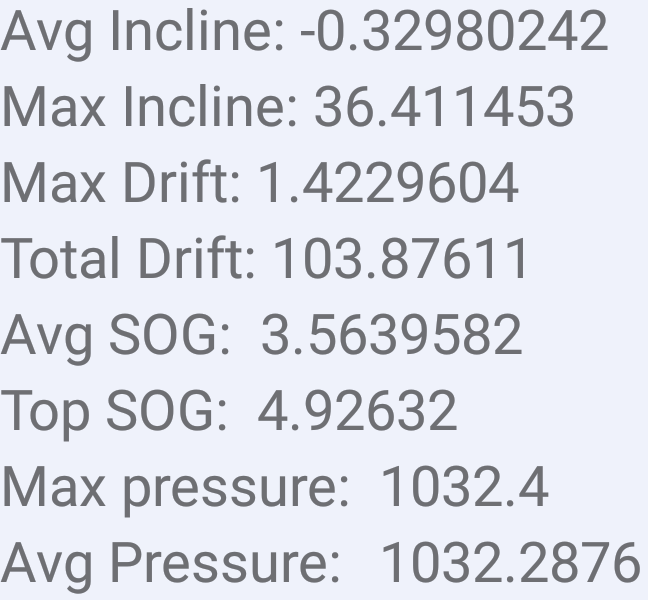
\includegraphics[width=\textwidth]{Figures/log_data.png}
	\caption{Log data summary example.}
	\label{log-summary}
	\end{minipage}
	~
	\begin{minipage}[t]{0.6\textwidth}
	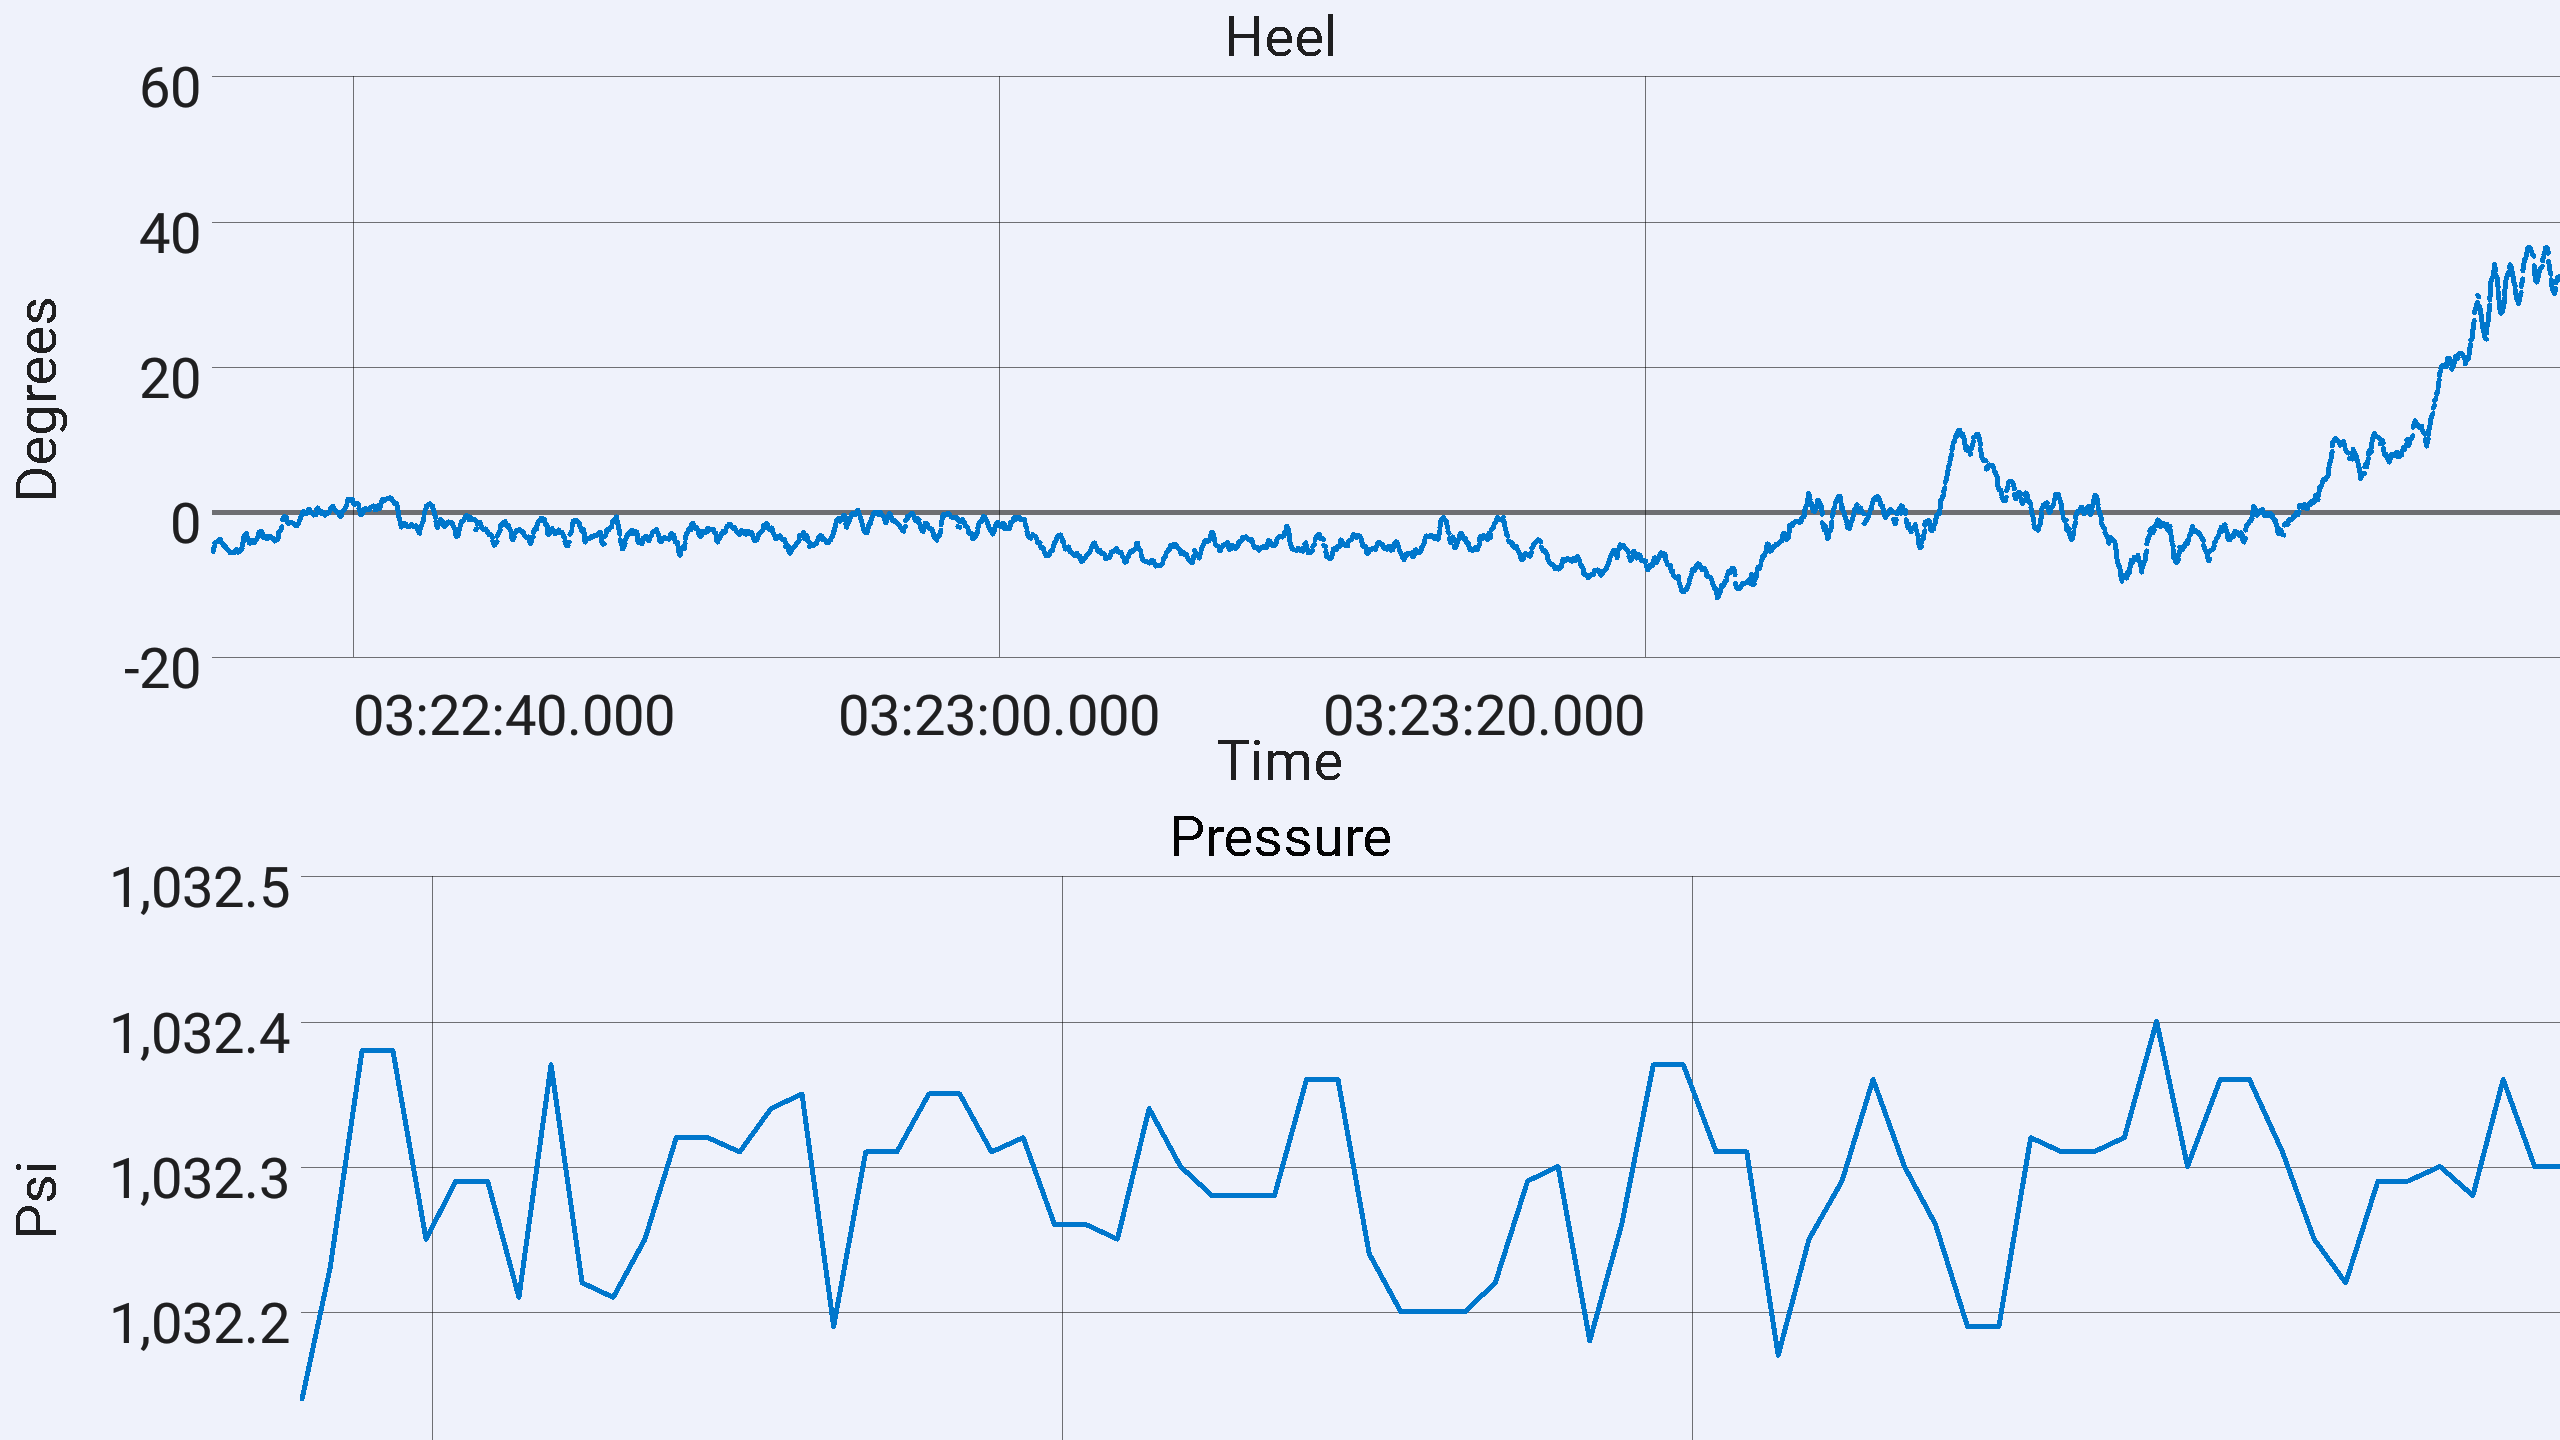
\includegraphics[width=\textwidth]{Figures/log_graph.png}
	\caption{Log graphs examples.}
	\label{log-graph}
	\end{minipage}
\end{figure}

\subsubsection{Bluethooth connection}
A list of all devices in the nearby area is displayed when the user decides to connect to the system, this adds flexibility to the user and allows for connection between multiple systems with different \gls{mac}. Scanning for nearby devices is done in the \emph{MainAcivity} and handled by the \emph{BTHandler} class. The application uses Bluetooth low energy technology to match the system implementation. This allows the device to receive notifications when the data is altered on the system and updates occurs in different frequencies for different types of data. To ensure a stable connection between the system and the device the connection class is implemented as an android service\cite{android-service}. This allows the device to keep the connection alive between different views and even when the device is put into sleep mode. All functionality regarding connecting and receiving data is implemented in the \emph{BTLEConnection} class and known characteristics and the determined unique GATT service identifiers are stored in the \emph{SampleGattAttributes} class.

\subsubsection{Map}
For the sailor to get more information about location two maps are implemented, one that is embedded into a layout in the \emph{FeedbackActivity} and the functionality of this is handled in the \emph{MapRunner} class, the other map is implemented in \emph{MapsActivity}. This could be improved by using the same class for both maps to achieve better readability and modifiability of the code. Both these implementations utilized the Google maps \gls{api}\cite{gmaps}, which can be used freely and the map service is highly accurate and suits our system well. Interaction with the maps can also be made quite easy which helped to make development faster. The sailor has the ability to see a path over the trip and the total distance traveled. Waypoints can be placed if the sailor wants to plan a certain trip in advance. The distance of the trip and the distance currently traveled is displayed to give the \gls{skipper} information on how long the trip is and how much of the trip is left to be sailed. A path to the nearest waypoint is shown to help navigation. When the sailor is close to the first waypoint the path to the next waypoint is shown. The waypoint route can also be viewed in the map of the \emph{FeedbackActivity} layout.

\subsubsection{Drift}
Calculating leeward drift is done by measuring the distance from an estimated destination point and the position received from the \gls{gps}. By using the \gls{gps} position and the ships bearing from the systems magnetometer a \textit{rhumb line}\cite{rhumb-line} is derived and the new estimated position is calculated with
%δ = d/R	(angular distance)
%φ2 = φ1 + δ ⋅ cos θ	
%Δψ = ln( tan(π/4 + φ2/2) / tan(π/4 + φ1/2) )	(‘projected’ latitude difference)
%q = Δφ/Δψ (or cos φ for E-W line)	
%Δλ = δ ⋅ sin θ / q	
%λ2 = λ1 + Δλ
\begin{align*}
  &\begin{aligned}
  \delta &= d/R 
  \end{aligned}\\
 &\begin{aligned}
  \varphi_2 &= \varphi_1 + \delta \cdot \cos{\theta}
  \end{aligned}\\
 &\begin{aligned}
  \Delta\psi = \ln { \bigg( \tan{\frac{n}{4} + \frac{\varphi_2}{2}} \bigg/ \tan{\frac{n}{4} + \frac{\varphi_1}{2}} \bigg)}
  \end{aligned}\\
 &\begin{aligned}
  q = \frac{\Delta\varphi}{\Delta\varphi}
  \end{aligned}\\
 &\begin{aligned}
  \Delta\lambda = \delta\cdot\sin\frac{\theta}{q}
  \end{aligned}\\
 &\begin{aligned}
  \lambda_2 = \Delta\lambda_1 + \Delta\lambda
  \end{aligned}\\
\end{align*}
where $R$ is the Earth's radius, $d$ is the distance traveled, $\theta$ is ships bearing, $\lambda_1$ and $\varphi_1$ is the point of origin in longitude and latitude. This new estimated position $\lambda_2$ and $\varphi_2$ is then compared to the next positional data from the \gls{gps} and the distance between these points is calculated using \emph{Equirectangular projection}\cite{equirectangular}.
%x = Δλ ⋅ cos φm
%y = Δφ
%d = R ⋅ √x² + y²
\begin{align*}
  &\begin{aligned}
  x = \Delta\lambda \cdot \cos\frac{\Delta\varphi}{2}
  \end{aligned}\\
 &\begin{aligned}
  y = \Delta\varphi
  \end{aligned}\\
 &\begin{aligned}
  d = R\cdot\sqrt{x^2+y^2}
  \end{aligned}\\
\end{align*}
where $\Delta\lambda$ and $\Delta\varphi$ are the differences in longitude and latitude for two location points. This function has high performance gain but is less accurate over large distances then, e.g., the \emph{Haversine formula}\cite{haversine}. Since for this function, only small changes in distance are calculated the accuracy is more than adequate. A problem with this way of calculating leeward drift is the accuracy of the \gls{gps} readings and to get a good bearing the idea was to make use of the magnetometer though the accuracy of that is also far from perfect. This combined with the fact that a small deviation of a couple of degrees results in a large drift resulted in large errors in leeway drift. The solution was to use the directional data sent from the \gls{gps} module which calculates direction based on last positional data. This solution works well for progress in the forward direction and when fast sideways motion is detected the estimated position will be along the same vector as the previous direction. However, for constant drift sideways this approach will display that no drift was taking place. This calculation is handled by the \emph{Locator} class.



























\clearpage
\section{Kalman filter}
\label{kf}
\chapterauthor{Axelsson, Oskar (no one)}
\subsection{Sensor theory}
Sensor fusion can be observed everywhere e.g., living animals uses all of its senses to survive daily, an animal cannot hunt using its eyes only, it has to combine its sense of smell, eyes, and hearing to hunt the prey\cite{animal}. Sensor fusion theory is not only found in the living species it is found in cars, planes, computers and so on, this to enhance performance and accuracy. In this project, a sensor fusion will be designed to enhance the accuracy of the dinghy's position and velocity. The fusion will be a global positioning system,  \gls{gps} and an \gls{ins}. The \gls{ins} uses a low priced \gls{imu}.\\ 
The \gls{gps}'s accuracy is not uniform since there might be building reflections, atmospherics delays or clock bias errors \cite{boken}. Using the only information provided by a \gls{sins} is not sufficient either since the \gls{imu} sensor will drift after time, but using the information provided by the \gls{ins} for short time intervals will give more accurate results.  

\subsection{Inertial Navigation System}
In navigation there exist different techniques on how to navigate using an \gls{imu}, a typical technique is using a \gls{sins}. A \gls{sins} consists of an \gls{imu} which is mounted on the dinghy so it measures the acceleration and rotational rate that the dinghy encounters.
The concepts of inertial navigation are to determine the position and velocity of the dinghy from a known starting point, using only measurements from the \gls{imu}. The \gls{imu}, in this case, consists of a three-axis gyroscope, a three-axis accelerometer, and a three-axis magnetometer. \\
Measurement from the gyroscope is to determine the angular motion of the dinghy, from that its heading relative to a reference frame can be derived.
By measuring specific forces acting on the dinghy using the accelerometer, then resolve the specific force measurements into the reference frame using the knowledge derived from the information provided by the gyroscope. 
The resolved specific force measurements are integrated to obtain its velocity and position. \cite{non-linear} 


\subsection{Sensor fusion}
A popular filter to use when applying sensor fusion is to use a Kalman filter. The Kalman Filter is a recursive filtering method for discrete data, the algorithm was developed by a Hungarian mathematician Rudolf (Rudi) Emil Kalman in 1960 \cite{boken}. It's popular to use due to its efficiency when calculating predictions. \cite{kf eff}

\subsection{Navigation Frames}
Navigation algorithm involves various coordinate frames and therefore transformation between frames is a must. In this case, four different frames is used.\\

The Inertial frame denoted $i$-frame for future notation is defined such that its origin is at the center of Earth and its axes $X_i$, $Y_i$ and $Z_i$ is non-rotating with respect to the stars. $Z_i$ is coincident with the Earth's polar axis, i.e. North.\\

The Earth navigation frame denoted $e$-frame for future notation is fixed with respect to Earth and has its origin at the center of the Earth. The frame is defined as $X_e$, $Y_e$ and $Z_e$, with $Z_e$ along Earth's polar axis. Axis $X_e$ and $Y_e$ lies along the intersection of the plane of the Greenwich meridian with the Earth's equatorial plane. The $e$-frame rotates at a constant rate with respect to the $i$-frame and is denoted $\omega_e$.\\

The Navigation frame denoted $n$-frame for future notation is a local frame and has its origin located in the navigation system, in this case, point P, see \autoref{WGS}, and its axes aligned with the directions of north, east and down, denoted NED. The turn rate of the navigation frame with respect to Earth's fixed frame, $\omega_{en}^n$, is directed by the motion of point P with respect to the Earth and is referred to the transport rate.   

\begin{figure}[H]
\centering
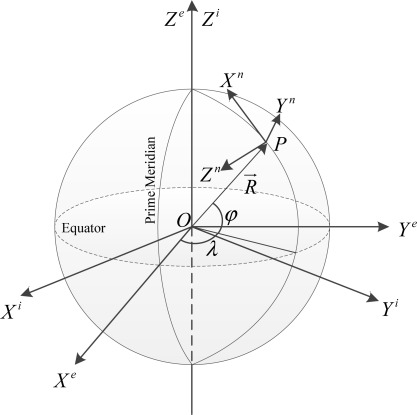
\includegraphics[width=0.3\textwidth]{Figures/WGS-coordinates.png}
\caption{Inertial, Earth and Navigation frame.}
\label{WGS}
\end{figure}

The Body frame denoted $b$-frame is the sensitive axes of the \gls{imu}'s sensors, which are made to coincide with the axes of the moving body in which the \gls{imu} is mounted in. The body, in this case, is referred to the dinghy, see \autoref{Fig:body_frame}.

\begin{figure}[H]
\centering
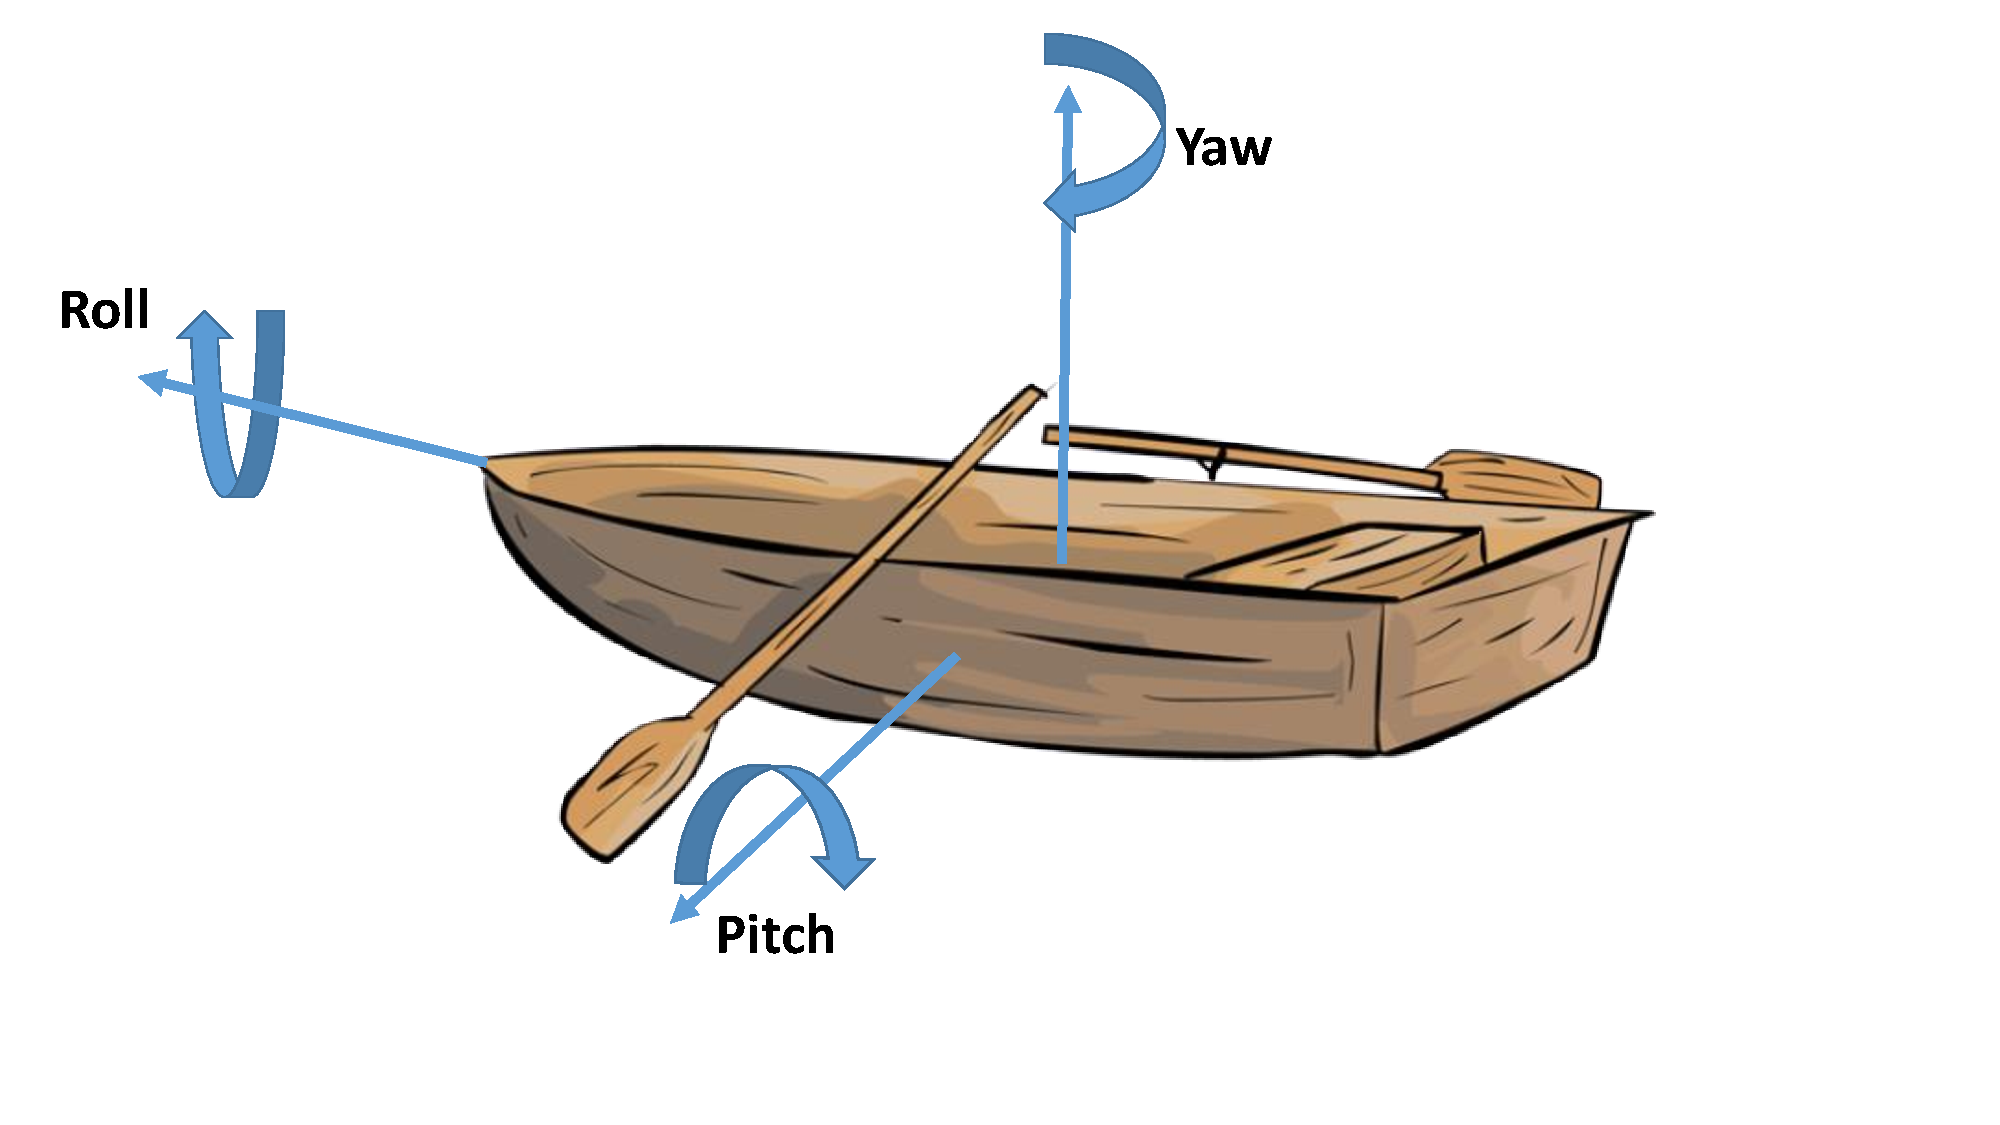
\includegraphics[width=0.5\textwidth]{Figures/Euler_angle.pdf}
\caption{Body frame.}
\label{Fig:body_frame}
\end{figure}
\begin{itemize}
\item Yaw $(\psi)$: Is an imaginary line running vertically through the ship and through its center of gravity. A yaw motion is a side-to-side movement of the bow and stern of the dinghy \cite{SNAME}.
\item Pitch $(\theta)$: Is an imaginary line running horizontally across the ship and through the center of gravity. A pitch motion is an up-or-down movement of the bow and stern of the dinghy \cite{SNAME}.
\item Roll $(\phi)$: Is an imaginary line running horizontally through the length of the ship, through its center of gravity, and parallel to the waterline. A roll motion is a side-to-side or port-starboard tilting motion of the superstructure around this axis\cite{SNAME}.
\end{itemize}

\subsection{Transformation Between Frames}
Referring to \autoref{WGS} it can be observed that its possible to align the $n$-frame with the $e$-frame, this is done by rotating the $n$-frame by ($\lambda-90$)-degrees around its $X$-axis (east-direction) and ($-\phi-90$)-degrees about its $Z$-axis, (downward direction) \cite{nonlinear}. Where $\lambda$ and $\varphi$ is the latitude and longitude, respectively. Then the transformation between the two frames can be done using the \gls{dcm}, which is defined as \cite{nonlinear}.
\begin{equation}
C_n^e=R_z(-\lambda-90)R_x(\varphi-90)
\label{Cosine_1}
\end{equation}
Where $C_n^e$ should be interpreted as moving from $n$-frame to $e$-frame, $R_x$ and $R_z$ are the rotation matrices around its axis, respectively. Expanding Eq. \eqref{Cosine_1} 
\begin{align}
C_n^e &=
\begin{bmatrix}
cos(-\lambda-90) & sin(-\lambda-90) & 0\\
-sin(-\lambda-90) & cos(-\lambda-90) & 0\\
0 & 0 & 1
\end{bmatrix}
\begin{bmatrix}
1 & 0 & 0\\
0 & cos(\varphi-90) & sin(\varphi-90) \\
0 & -sin(\varphi-90) & con(\varphi-90) \\
\end{bmatrix}\\
C_n^e &=
\begin{bmatrix}
-sin(\lambda) & -cos(\lambda) & 0\\
cos(\lambda) & -sin(\lambda) & 0\\
0 & 0 & 1
\end{bmatrix}
\begin{bmatrix}
1 & 0 & 0\\
0 & sin(\varphi) & -cos(\varphi) \\
0 & sin(\varphi) & sin(\varphi) \\
\end{bmatrix}\\
C_n^e &=
\begin{bmatrix}
-sin(\lambda) & -sin(\varphi)cos(\lambda) & cos(\varphi)cos(\lambda) \\
cos(\lambda) & -sin(\varphi)sin(\lambda) &  cos(\varphi)sin(\lambda) \\
0 & cos(\varphi) & sin(\varphi) \\
\end{bmatrix}
\end{align}
Exploring the orthogonality its possible to transform from $e$-frame to $n$-frame by taking the inverse of the equation above, i.e.
\begin{equation}
(C_n^e)^{-1}=C_e^n
\label{Eq.Earth2Nav}
\end{equation}
Using Eq. \eqref{Eq.Earth2Nav} its now possible to move from $e$-frame to $n$-frame. \\


Transforming from $n$-frame to $b$-frame is done in the same way, i.e. using rotation matrices. The \gls{dcm}, moving from $b$-frame to $n$-frame is given by \cite{nonlinear}
\begin{equation}
C_b^n=R_z(-\psi)R_y(-\theta)R_x(-\phi),
\label{Body_rotation}
\end{equation}
where 
\begin{align}
R_z(-\psi) = &
\begin{bmatrix}
cos(\psi) & -sin(\psi) & 0\\
sin(\psi) & cos(\psi) & 0 \\
0 & 0 & 1
\end{bmatrix}\label{R_z} \\
R_y(-\theta) = &
\begin{bmatrix}
cos(\theta) & 0 & sin(\theta)\\
0 & 1 & 0 \\
-sin(\theta) & 0 & cos(\theta)
\end{bmatrix}\label{R_y} \\
R_x(-\phi) = &
\begin{bmatrix}
1 & 0 & 0\\
0 & cos(\phi) & -sin(\phi)\\
0 & sin(\phi) & cos(\phi)
\end{bmatrix}\label{R_x}
\end{align}
Solving Eq. \eqref{Body_rotation} with \eqref{R_z}, \eqref{R_y} and \eqref{R_x}
\begin{align}
C_b^n = &
\begin{bmatrix}
cos(\psi) & -sin(\psi) & 0\\
sin(\psi) & cos(\psi) & 0 \\
0 & 0 & 1
\end{bmatrix}
\begin{bmatrix}
cos(\theta) & 0 & sin(\theta)\\
0 & 1 & 0 \\
-sin(\theta) & 0 & cos(\theta)
\end{bmatrix}
\begin{bmatrix}
1 & 0 & 0\\
0 & cos(\phi) & -sin(\phi)\\
0 & sin(\phi) & cos(\phi)
\end{bmatrix}
\label{expand_Body_rotation} \\ \\
C_b^n  = & 
\begin{bmatrix}
cos(\theta)cos(\psi) & -cos(\phi)sin(\psi)+sin(\phi)sin(\theta)cos(\psi) &  sin(\phi)sin(\psi)+cos(\phi)sin(\theta)cos(\psi) \\
cos(\theta)sin(\psi) & cos(\phi)cos(\psi)+sin(\phi)sin(\theta)sin(\psi) & -sin(\phi)cos(\psi)+cos(\phi)sin(\theta)sin(\psi)\\
-sin(\theta) & sin(\phi)cos(\theta) & cos(\phi)cos(\theta) 
\end{bmatrix}
\end{align}
Where $\psi$, $\theta$ and $\phi$ are the Euler angles as described earlier. Expressing the matrix above in a more compact form.
\begin{align}
C_b^n = &
\begin{bmatrix}
c_{11} && c_{12} && c_{13}\\
c_{21} && c_{22} && c_{23} \\
c_{31} && c_{32} && c_{33}
\end{bmatrix}
\label{Eq.C_b_n_compact}
\end{align}
The Euler angles is a transformation from one coordinate frame to another and is defined by three successive rotations about the different axis. Its possible to see the three angles as a set of mechanical gimbals. 
The problem with Euler angles is that when rotating about each axis, its possible to drive two of the three gimbals so they appear parallel to each other this implies that a degree of freedom is lost, this is called a gimbal-lock \cite{nonlinear}. To resolve this issue its possible to use quaternion attitude representation instead, as Euler angels the representation allows transformation between one coordinate frame to another, but the difference is that the transformation is done in a single rotation, instead of three about a vector defined in the reference frame. The \gls{dcm} using quaternion is defined such that\cite{nonlinear}
\begin{align}
C_b^n & =
\begin{bmatrix}
(q_1^2 + q_2^2 - q_3^2-q^4) && 2(q_2q_3 - q_1q_4) && 2(q_2q_4 + q_1q_3) \\
2(q_2q_3 - q_1q_4) && (q_1^2 - q_2^2 + q_3^2-q^4) && 2(q_3q_4 - q_1q_2) \\
2(q_2q_4 - q_1q_3) && 2(q_3q_4 + q_1q_2) && (q_1^2 - q_2^2 - q_3^2+q^4)
\end{bmatrix}
\end{align}

Where $q_1$, $q_2$, $q_3$ and $q_4$ can be derived using the Euler angles from \autoref{Eq.C_b_n_compact}
\begin{align*}
q_1 =& \frac{1}{2}(1+c_{11} + c_{22} + c_{33})^{0.5} \\
q_2 =& \frac{1}{4q_1}(c_{32} - c_{23})\\
q_3 =& \frac{1}{4q_1}(c_{13} - c_{31})\\
q_4 =& \frac{1}{4q_1}(c_{21} - c_{12})\\
\end{align*}


The angular velocity of the $e$-frame with respect to the $i$-frame projected onto the $e$-frame is given as \cite{nonlinear}
\begin{equation}
\bar{\omega}_{ie}^e = 
\begin{bmatrix}
0 & 0 & \omega_e
\end{bmatrix}^T.
\end{equation}
Where $\omega_e$ is the angular velocity of the Earth and has a value of
$7.2921158 \times 10^{-5}$ $rad/s$ \cite{nonlinear}. Using the projection matrix Eq. \eqref{Cosine_1} its possible to project $\bar{\omega}_ {ie}^i$ onto the $n$-frame
\begin{align}
\bar{\omega}_{ie}^n=C_e^n\bar{\omega}_{ie}^e=
\begin{bmatrix}
\omega_e cos(\varphi) & 0 & -\omega_e sin(\varphi)
\end{bmatrix}^T.
\label{omega_ie}
\end{align}
$\bar{\omega}_{en}^n$ represents the turn rate of the $n$-frame with respect to the $e$-frame its called the transport rate and may be expressed as the rate of change of latitude and longitude as follows
\begin{align}
\bar{\omega}_{en}^n=
\begin{bmatrix}
\dot{\lambda}cos(\varphi) & -\dot{\varphi} & -\dot{\lambda}sin(\varphi)
\end{bmatrix}^T.
\label{omega_en}
\end{align}
Where $\dot{\lambda}=v_e/(R_N+h)cos(\varphi)$ and $\dot{\varphi}=v_n/(R_E+h)$ \cite{nonlinear}, here we assume the Earth to be an ellipsoid and that there are no variations in Earth's gravitation depending on where the user is on the ellipsoid. $R_N$ is the meridian radius of curvature and defined as $R_N=R_0(1-e^2)/(1-e^2sin^2\varphi)^{3/2}$ \cite{nonlinear}. $R_E$ is the transverse radius of curvature and defined as $R_E=R_0/(1-e^2sin^2\varphi)^{1/2}$. Where $R_0$ is the length of the semi-major axis and has a constant value of $6356752.3142$ m, $e$ is the major eccentricity of the ellipsoid and has a constant value of $0.081819$, $\varphi$ is the current latitude in radians, $v_N$ and $v_E$ is the velocity in north and east direction, respectively and $h$ is the height above the surface of the Earth. Then Rewriting Eq. \eqref{omega_en} with the new expressions.
\begin{align}
\bar{\omega}_{en}^n=
\begin{bmatrix}
v_e/(R_E+h) & -v_n/(R_N+h) & -v_e tan(\varphi)/(R_N+h)
\end{bmatrix}^T \label{omega_en_ny}
\end{align}
Now the turn rate of the $n$-frame with respect to $i$-frame, $\bar{\omega}_{in}^n$ can be obtained by adding Eq. \eqref{omega_ie} and \eqref{omega_en_ny} together.
\begin{align}
\bar{\omega}_{in}^n=
\begin{bmatrix}
\omega_e cos(\varphi) + v_e/(R_E+h) & v_n/(R_N+h) & -\omega_e sin(\varphi) + v_e tan(\varphi)/(R_N+h)
\end{bmatrix}^T
\label{Eq.omega_in}
\end{align}

\noindent Now Eq. \eqref{Eq.omega_in} is a function dependent both on velocity and position.

\subsection{Inertial Navigation Equation}
Describing the position of the dinghy in the $n$-frame is done by \cite{nonlinear}.
\begin{align}
\bar{r}^n=
\begin{bmatrix}
\varphi & \lambda & h
\end{bmatrix}^T.
\end{align}
Since velocity is described as the rate of change of its position with respect to a frame of reference and is a function of time, the velocities in the north, east and down can be expressed as.
\begin{align}
\begin{bmatrix}
v_N \\
v_E \\
v_D
\end{bmatrix}
=
\begin{bmatrix}
(R_E+h) & 0 & 0 \\
0 & (R_N+h)cos(\varphi) & 0\\
0 & 0 & -1
\end{bmatrix}
\begin{bmatrix}
\dot{\varphi}\\
\dot{\lambda}\\
\dot{h}
\end{bmatrix}
\label{Eq.v_n1}
\end{align}
Where $\dot{-}$ symbolizes the first derivative with respect to time. Thus, $\dot{\varphi}$, $\dot{\lambda}$ and $\dot{h}$ can be derived by rewriting Eq. \eqref{Eq.v_n1} as

\begin{align}
\begin{bmatrix}
\dot{\varphi}\\
\dot{\lambda}\\
\dot{h}
\end{bmatrix}
=
\underbrace{\begin{bmatrix}
\frac{1}{(R_E+h)} & 0 & 0 \\
0 & \frac{1}{(R_N+h)cos(\varphi)} & 0\\
0 & 0 & -1
\end{bmatrix}}_{D^{-1}}
\begin{bmatrix}
v_N \\
v_E \\
v_D
\end{bmatrix}
\label{Eq.v_n}
\end{align}

\noindent Thus the dynamics describing the system can be expressed as \cite{nonlinear}.

\begin{align}
\dot{\bar{r}}_n = & D^{-1}v_n
\label{Eq.r_n_t}\\
\dot{\bar{v}}_n = & C_b^n \bar{f}^b-(2\omega_{ie}^n+\omega_{en}^n) \times \bar{v}_n +\bar{g}^n
\label{Eq.v_n_t}\\
\dot{C}_b^n = & C_b^n(\Omega_{ib}^b - \Omega_{in}^b)
\label{Eq.C_b_n_t}
\end{align}
Where $\bar{f}^b$ is the specific force vector defined as the difference between the true acceleration in
space and the acceleration due to gravity and $\bar{g}^n$ is the gravity vector. Where $\Omega$ is the skew matrix of $\omega$, more precise $\Omega_{ib}^b$ the skew-matrix of the outputs of the strapdown gyroscopes and $\Omega_{in}^n$ is the skew-matrix of Eq. \eqref{Eq.omega_in}. Skew-matrix is defined as the cross product between the vectors.


\subsection{INS mechanization}
Since the INS has to work in discrete time domain, Eq. \eqref{Eq.r_n_t}, \eqref{Eq.v_n_t} and \eqref{Eq.C_b_n_t} has to be discretized. The sampling time should be seen as a changing variable since it may not be constant instead it will fluctuate around $100Hz$, this means that $\Delta t_k = \Delta k_{k-1} - t_{k}$, this to improve the accuracy. The discrete dynamics are \cite{non-linear}, Using Eq. \eqref{Eq.r_n_t},\eqref{Eq.v_n_t} and \eqref{Eq.C_b_n_t}.


\begin{align}
\bar{r}_{k+1}^n = & \bar{r}_k + 0.5D^{-1}(\bar{v}_k^n + \bar{v}_{k+1}^n)\Delta t
\label{Eq.r_n_d}\\
v_{k+1}^n= & \bar{v}_k + \Delta \bar{v}_{k+1}^n
\label{Eq.v_n_d}\\
\dot{C}_b^n = & C_b^n(\Omega_{ib}^b - \Omega_{in}^b)\Delta t
\label{Eq.C_b_n_d}
\end{align}
where 
\begin{equation}
\Delta \bar{v}_{k+1}^n = \Delta \bar{v}_f^n - (2\omega_{ie}^n+\omega_{en}^n) \times \bar{v}_n \Delta t +\bar{\gamma}\Delta t
\end{equation}
where $\gamma = [0 \quad 0 \quad 9.8123]$.\\ \\
The Navigation frame Inertial Navigation System can now be seen in \autoref{Fig:body_frame}, Where its possible to examine all the steps which were derived earlier, from the \gls{imu} to the output.
\begin{figure}[H]
\centering
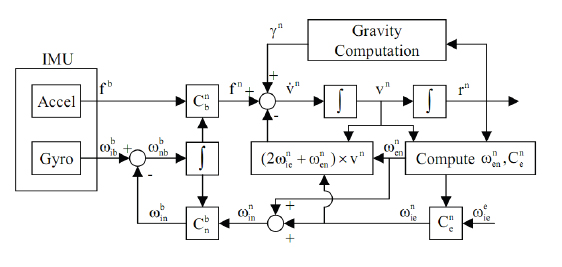
\includegraphics[width=\textwidth]{Figures/ins_2.jpg}
\caption{The Inertial Navigation Frame.}
\label{Fig:body_frame}
\end{figure}
\section{Implementation of Sensor Fusion Using a Kalman Filter.}
\subsection*{Perturbation Analysis}
Since the differential equations describing velocity, position, and the attitude, \gls{dcm} are non-linear, utilize a perturbation series to minimize the errors \cite{pertubation}.
\begin{equation}
\hat{r}^n =r^n+\delta r^n
\label{Eq.per_r}
\end{equation}
\begin{equation}
\hat{v}^n =v^n+\delta v^n
\label{Eq.per_v}
\end{equation}
\begin{equation}
\hat{C}_b^n = (I-E^n)C_b^n
\label{Eq.per_c}
\end{equation}
Where $E^n$ is the skew matrix and given as.
\begin{align}
\begin{bmatrix} 
0 && -e_D && e_E \\
e_D && 0 && -e_N \\
-e_E && e_N && 0
\end{bmatrix}
\end{align}
Where $\hat{}$ is the computed values, $\delta$ and $e_{NED}$ are the errors in North, East and upward direction, respectively.

\subsubsection{Error Dynamics Position}
Perturbing \eqref{Eq.per_r}, the linearized position is obtained since the position dynamics is a function of both position and velocity, the position error dynamics is obtained as
\begin{equation}
\delta \dot{\bar{r}}^n = F_{rr}\delta \bar{r}^n + F_{rv}\delta \bar{v}^n.
\end{equation}

\noindent Where
\begin{align}
F_{rr} &=
\begin{bmatrix}
0 && 0 && \frac{-v_N}{(M+h)^2}\\
\frac{v_E sin(\varphi)}{(N+h)cos^2(\varphi)} && 0 && \frac{-v_E}{(N+h)^2cos(\varphi)} \\
0 && 0 && 0
\end{bmatrix}
\label{Eq.Frr}
\end{align}
and
\begin{align}
F_{rv} &=
\begin{bmatrix}
\frac{1}{(M+h)} && 0 && 0\\
0 && \frac{1}{(N+h)cos(\varphi)} && 0 \\
0 && 0 && -1
\end{bmatrix}.
\label{Eq.Frv}
\end{align}
\subsubsection{Error Dynamics Velocity}
The same is used when deriving the perturbation for the velocity, Eq. \eqref{Eq.per_v}, here, velocity is described by forces and gravity acting on the dinghy. Using Eq. \eqref{Eq.v_n_t}, and perturbation Eq. \eqref{Eq.per_v}, the following is obtained \cite{nonlinear}.
\begin{equation}
\delta \dot{\bar{v}}^n = \bar{v}_n \times \underbrace{(2\delta \bar{\omega}_{ie}^n+ \delta \bar{\omega}_{en}^n)}_{I}+\delta \bar{g}^n -\underbrace{(2\bar{\omega}_{ie}^n + \bar{\omega}_{en}^n)}_{II}\times \delta \bar{v}^n + (\bar{f}^n\times) e^n +C_b^n\delta \bar{f}^n
\label{Eq.delta_v}
\end{equation}
where $II$ is expressed as follow, using Eq. \eqref{Eq.omega_in}.
\begin{align}
2\bar{\omega}_{ie}^n + \bar{\omega}_{en}^n = 
\begin{bmatrix}
2\omega_e cos(\varphi) + \frac{v_E}{(N+h)} \\
\frac{-v_N}{(M+h)} \\
-2\omega_e sin(\varphi) - \frac{v_E tan(\varphi)}{(N+h)}
\end{bmatrix}.
\label{Eq.II}
\end{align}
Now perturbing $I$ with $II$, using Eq. \eqref{omega_en} and \eqref{Eq.omega_in}, the following is obtained.
\begin{align}
2\delta \bar{\omega}_{ie}^n+ \delta \bar{\omega}_{en}^n =
\delta \Omega_r\delta \bar{r}^n + \delta\Omega_r\delta\bar{v}^n
\end{align}
where
\begin{align}
\delta\Omega_r = 
\begin{bmatrix}
-2 \omega_e sin(\varphi) && 0 && \frac{-v_E}{(N+h)^2}\\
0 && 0 && \frac{v_N}{(M+h)^2}\\
2 \omega_e cos(\varphi)-\frac{v_E}{(N+h)cos^2(\varphi)} && 0 && \frac{v_E tan(\varphi)}{(N+h)^2}
\end{bmatrix}
\label{Eq.Omega_r}
\end{align}
and
\begin{align}
\delta\Omega_v = 
\begin{bmatrix}
0 &&  \frac{-1}{(N+h)} && 0\\
\frac{-1}{(M+h)} && 0 && 0\\
0 && \frac{-tan(\varphi)}{(N+h)} && \frac{v_E tan(\varphi)}{(N+h)^2}
\end{bmatrix}
\label{Eq.Omega_v}
\end{align}
Then calculating the first term on the left side of Eq. \eqref{Eq.delta_v}, using Eq. \eqref{Eq.Omega_r} and \eqref{Eq.Omega_v}
\begin{align}
\bar{v}^n\times(2\delta \bar{\omega}_{ie}^n+\delta \bar{\omega}_{en}^n) = 
\bar{v}^n \times \delta\Omega_r\delta\bar{r}^n +\bar{v}^n\times\delta\Omega_v\delta\bar{v}^n
\end{align}
Then expressing Eq. \eqref{Eq.delta_v} as
\begin{equation}
\delta\bar{v}^n = F_{vr}\delta\bar{r}^n + F_{vv}\delta\bar{v}^n + (\bar{f}^n	\times)\bar{e}^n + C_n^b\delta \bar{f}^b
\end{equation}
Expressing $F_{vr}$ and $F_{vv}$ in matrix notation
\begin{align}
F_{vr} = 
\begin{bmatrix}
-2v_E\omega_e cos(\varphi)-\frac{v_E^2}{(N+h)cos^2(\varphi)} && 0 && \frac{-v_N v_D}{(M+h)^2} + \frac{v_E^2 tan(\varphi)}{(N+h)^2} \\
2\omega_e(v_N cos(\varphi)-v_D sin(\varphi)) + \frac{v_Ev_N}{(N+h)cos^2(\varphi)} && 0 && \frac{-v_E v_D}{(N+h)^2} - \frac{v_Nv_E tan(\varphi)}{(N+h)^2} \\
2v_E\omega_e sin(\varphi) && 0 && \frac{v_E^2}{(N+h)^2} + \frac{v_N^2}{(M+h)^2} - \frac{2\gamma}{R+h}
\end{bmatrix}
\label{Eq.Fvr}
\end{align}
and
\begin{align}
F_{vv} = 
\begin{bmatrix}
\frac{v_D}{(M+h)} && -2\omega_e sin(\varphi) -2\frac{v_Etan(\varphi)}{(N+h)} && \frac{v_N}{(M+h)} \\
2\omega_e sin(\varphi) +\frac{v_E tan(\varphi)}{(N+h)} && \frac{v_D + v_N tan(\varphi)}{(N+h)} && 2\omega_e cos(\varphi)+ \frac{v_E}{(N+h)} \\
-2\frac{v_N}{(M+h)} && -2\omega_e cos(\varphi) -2\frac{v_E}{(N+h)} && 0
\end{bmatrix}
\label{Eq.Fvv}
\end{align}
\subsubsection{Error Dynamics Attitude}
The output from the \gls{ins} can be expressed using Eq. \eqref{Eq.C_b_n_t}.
\begin{equation}
\hat{\dot{C}}_b^n = \hat{C}_b^n(\hat{\Omega}_{ib}^b - \hat{\Omega}_{in}^b)
\end{equation}
Then relate the above equation with Eq. \eqref{Eq.per_c}
\begin{equation}
-\dot{E}^nC_b^n = (I_E^n)C_b^n(\delta\Omega_{ib}^b-\delta\Omega_{in}^b)
\end{equation}
Expressing $\dot{E}^n$ by is self in left-hand side, the equation above can be expressed as
\begin{equation}
\dot{E}^n = -C_b^n(\delta\Omega_{ib}^b-\delta\Omega_{in}^b)
\end{equation}
or in vector form
\begin{equation}
\dot{\bar{e}}^n = -C_b^n(\delta\omega_{ib}^b-\delta\omega_{in}^b).
\label{Eq.error_vec}
\end{equation}

Since we want to express the equation above in its error equation $\delta \bar{\omega}_{in}^b$, the following change can be done $\hat{\bar{\omega}}_{in}^b = \hat{C}_n^b\hat{\bar{\omega}}_{in}^n$ This can be expanded into
\begin{equation}
\bar{\omega}_{in}^b + \delta \bar{\omega}_{in}^b = C_b^n(I+E^n)(\bar{\omega}_{in}^n+\delta\bar{\omega}_{in}^n).
\end{equation}
Using vector notation for the skew matrix, the equation above can be written as
\begin{equation}
\delta\bar{\omega}_{in}^b = C_n^b [\delta\bar{\omega}_{in}^n + (e^n\times)\bar{\omega}_{in}^n].
\label{Eq.del_omega}
\end{equation}
Substituting Eq. \eqref{Eq.del_omega} into Eq. \eqref{Eq.error_vec}, the following is obtained

\begin{equation}
\dot{\bar{e}}^n = \delta\bar{\omega}_{in}^n -(\bar{\omega}_{in}^n \times )\bar{e}^n - C_b^n\delta \bar{\omega}_{ib}^b 
\label{Eq.err_final}
\end{equation}
Then expressing the first term on the right-hand side into the position and velocity error terms explicitly, using Eq. \eqref{Eq.v_n} and \eqref{Eq.II}. The error attitude dynamics is then obtained and written as
\begin{equation}
\dot{\bar{e}}^n = F_{er}\delta \bar{r}^n + F_{ev}\delta \bar{v}^n - (\bar{\omega}_{in}^n \times)\bar{e}^n - C_b^n\delta\bar{\omega}_{ib}^b.
\end{equation}
Where $F_{er}$ and $F_{ev}$ is	
\begin{align} = 
F_{er} =
\begin{bmatrix}
-\omega_e sin(\varphi) && 0 && \frac{-v_E}{(N+h)^2}\\
0 && 0 && \frac{v_N}{(M+h)^2} \\
\omega_e cos(\varphi) - \frac{v_E}{(N+h)cos^2(\varphi)} && 0 && \frac{v_E tan(\varphi)}{(N+h)^2}
\end{bmatrix}
\label{Eq.Fer}
\end{align}

\begin{align} = 
F_{ev} =
\begin{bmatrix}
0 && \frac{1}{(N+h)} && 0\\
\frac{-1}{(M+h)} && 0 && 0\\
0 && \frac{-tan(\varphi)}{(N+h)} && 0
\end{bmatrix}.
\label{Eq.Fev}
\end{align}

\subsection{Implementing the Fusion Kalman Filter}
This system uses a feedback method to control the drift errors in the \gls{imu}, the model can be seen in \autoref{Fig:Feedback}.
\begin{figure}[H]
\centering
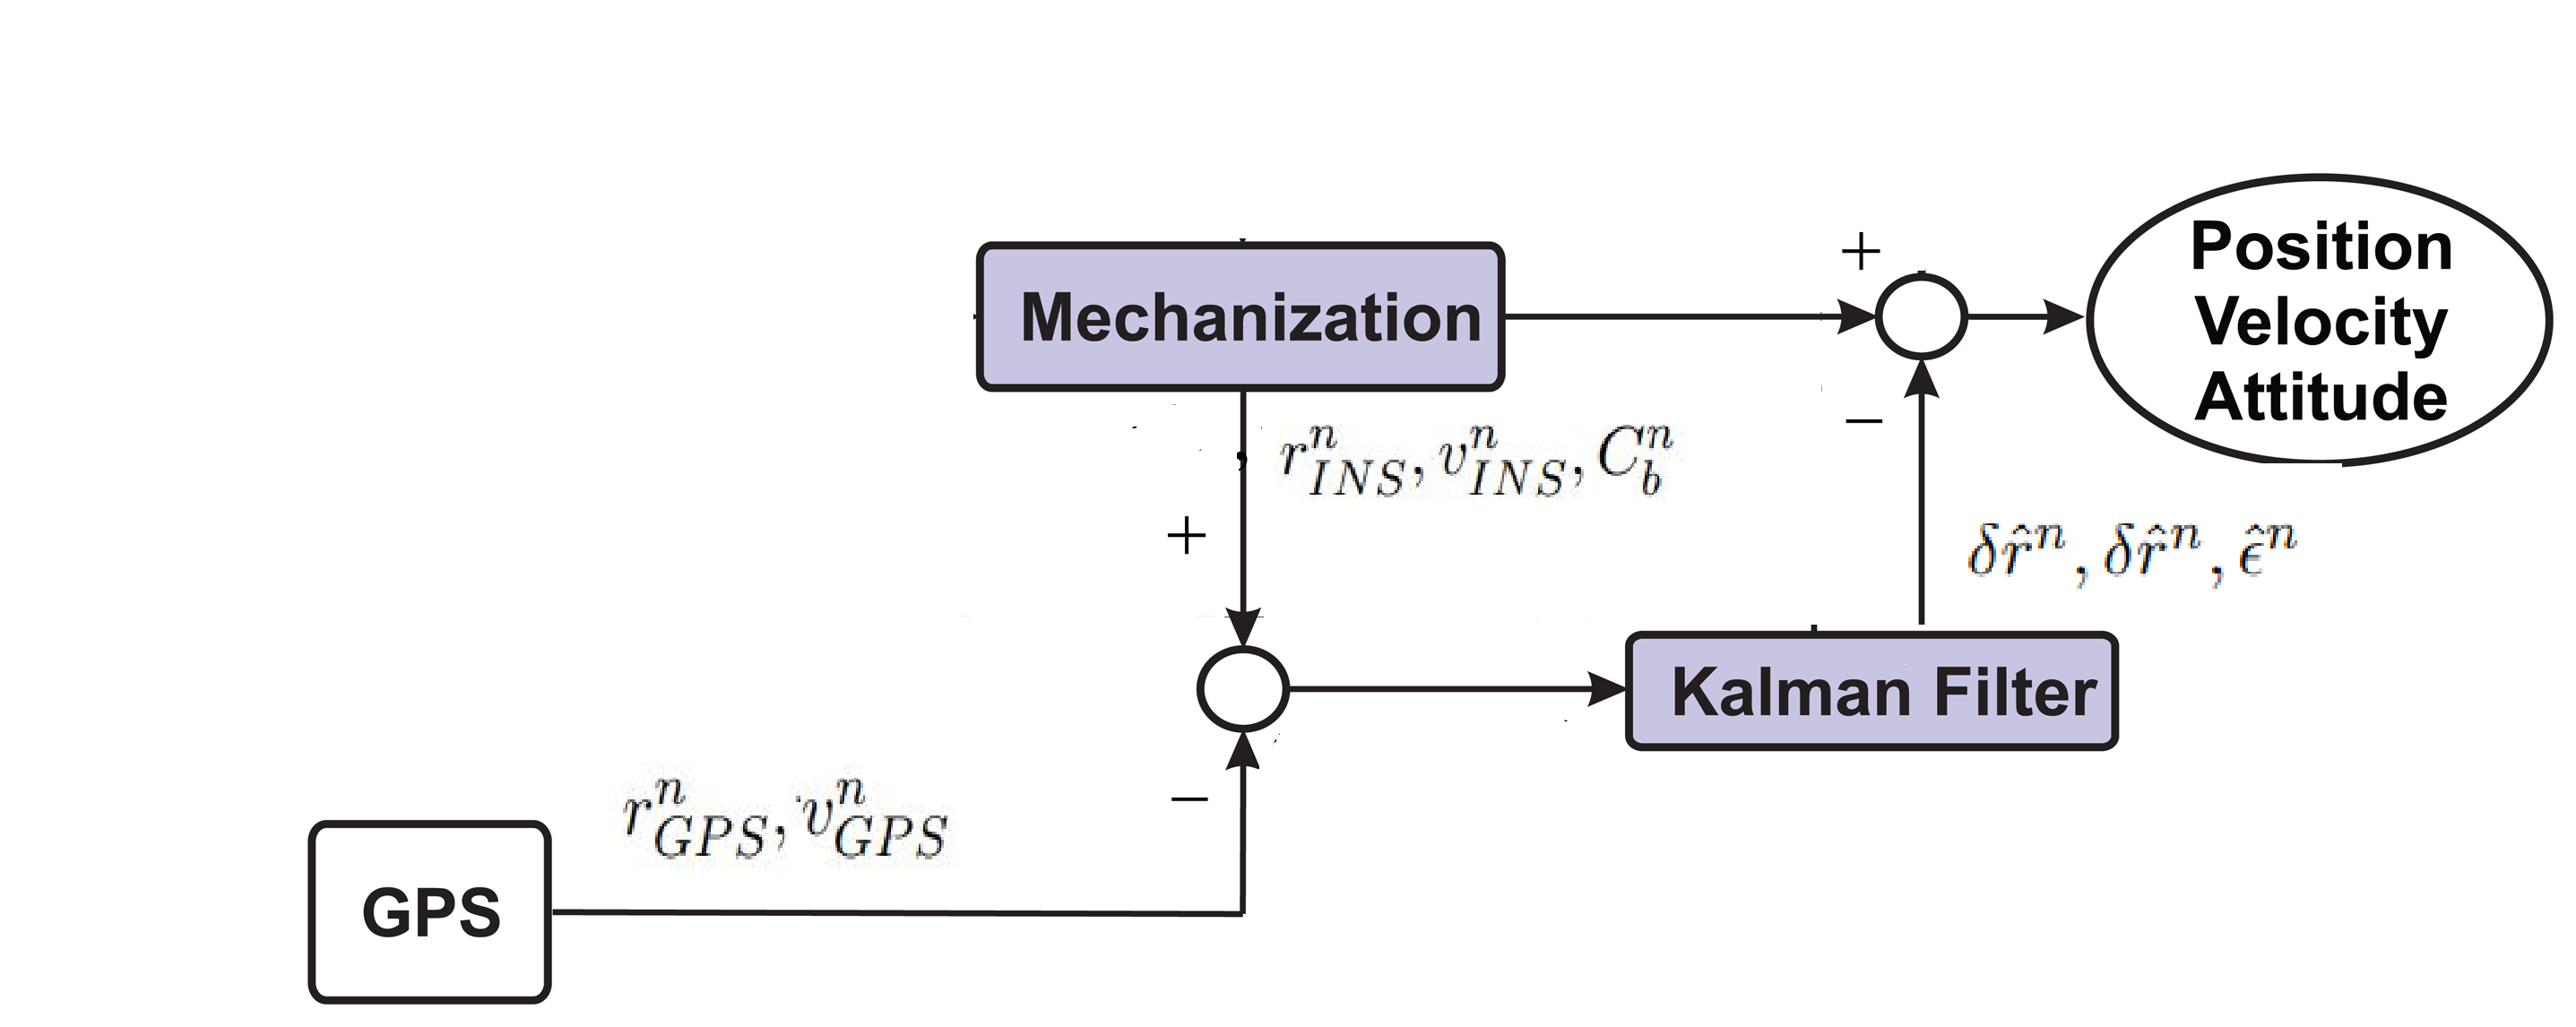
\includegraphics[width=0.7\textwidth]{Figures/feed-back.png}
\caption{The feedback-method which is used in the system.}
\label{Fig:Feedback}
\end{figure}
Implementing a continuous Kalman Filter using integration between Inertial Navigation System and a Global Positioning System.
\begin{align}
\hat{\bar{x}} = F \bar{x} + G \bar{u}
\label{eq.state_1}
\end{align}
Where $F$ is describing the dynamics of the system, $\bar{x}$ is the state vector, $G$ is the design matrix, $\bar{u}$ is the input matrix, i.e. forces acting on the dinghy recorded by the \gls{imu} and $\hat{\bar{x}}$ is the estimated state vector. \\

Where $F$ is a $9\times 9$ matrix and contain Eq. \eqref{Eq.Frr}, \eqref{Eq.Frv}, \eqref{Eq.Fvr}, \eqref{Eq.Fvv}, \eqref{Eq.Fer}, \eqref{Eq.Fev}, \eqref{Eq.omega_in}, and $\bar{x}$ is a $9 \times 1$ is given by
\begin{align}
F=
\begin{bmatrix}
F_{rr} & F_{rv} & 0 &\\
F_{vr} & F_{vv} & (\bar{f}^n \times)\\
F_{er} & F_{ev} & -(\bar{\omega}_{in}^n\times)
\end{bmatrix},
\qquad
\bar{x}=
\begin{bmatrix}
\delta\bar{r}^n \\
\delta\bar{v}^n\\
\delta\bar{e}^n
\end{bmatrix}
\end{align}
$G$ is a $6\times6$ matrix and $\bar{u}$ is a $6 \times 1$ vector and is defined as.
\begin{align}
G=
\begin{bmatrix}
-C_b^n & 0 \\
0 & C_b^n
\end{bmatrix},
\qquad
\bar{u}=
\begin{bmatrix}
\delta \bar{\omega}_{ib}^b \\
\delta \bar{f}^b 
\end{bmatrix}
\end{align}
The elements of $\bar{u}$ is assumed to be white noise with zero mean, thus
\begin{align}
Q=diag
\begin{bmatrix}
\sigma^2_{ax} & \sigma^2_{ay} & \sigma^2_{az} & \sigma^2_{gx} & \sigma^2_{gy} & \sigma^2_{gz}
\end{bmatrix}^T
\label{Eq.Q}
\end{align}
where $\sigma^2_{a(x,y,z)}$ and $\sigma^2_{g(x,y,z)}$ is the variance for the accelerometer and gyroscope in every direction, respectively.\\
	
Since a computer does not use continuous time domain the equation has to be transformed into discrete domain. The state equation will then be expressed as
\begin{equation}
\hat{\bar{x}}_{k+1} = \Phi_k \bar{x}_k +  \bar{w}_k	
\label{Eq.discrete}
\end{equation}
Here $\Phi_k$ is the state transition matrix in discrete time domain, in order to obtain a discrete state transition matrix the inverse Laplace transform is performed on the continuous state transition matrix, i.e.
\begin{equation}
\Phi_k = \mathcal{L}^{-1}\big[(SI-F)^{-1}\big]
\label{Eq.Phik}
\end{equation}
Since the sample interval, $\Delta t$ is very small in this case Eq. \eqref{Eq.Phik} can be approximated using Taylor approximation 
\begin{equation}
\Phi_k = e^{F\Delta t} \approx I + F \Delta t 
\label{Eq.Final_Phik}.
\end{equation}
From Eq. \eqref{Eq.discrete}, $\hat{w}_k$ is the driven response $t_{k+1}$ due to the input white noise. White noise is uncorrelated between sample periods, i.e the noise between $t_k$ and $t_{k+1}$ is uncorrelated \cite{signal_process}. Then the covariance matrix which is associated with $\bar{w}_k$ is \cite{signal_process}

\begin{align}
\mathbb{E}[\bar{w_i}\bar{w}_j^T] =
\begin{cases}
  Q_k &\quad i=j\\    
  0 &\quad i\neq j   
\end{cases}
\end{align}

and $Q_k$ can then be approximated using a first order of the discrete transition matrix \cite{Discrete_kalman}
\begin{equation}
Q_k\approx \Phi_k GQG^T \Phi_k^T.
\label{Eq.Q_k}
\end{equation}

If Eq. \eqref{Eq.Q} is analyzed, by increase the norm of $Q_k$ the Kalman Filter trusts the measurements more than the system, which will make the output more noisy due to noise induced from the measurements, the advantages with a large norm is that the time lag will decrease. If the norm is small the measurements will be less induced by measurement noise but time lag will increase, which means that we don't trust the measurements. Determining $Q_k$ can be done by testing several different settings and from that make an assumption, but a good assumption should be that the trajectory of the output should follow the \gls{gps} data when the \gls{gps} is connected to several satellites.\\



The Kalman filter is a linear quadratic estimator which is recursive and the estimator is unbiased and has minimum variance. The algorithm starts with a random process model, i.e. Eq. \eqref{Eq.discrete} and the following observation matrices \cite{Discrete_kalman}.

\begin{equation}
z_k = H_k\bar{x}_k + \bar{e}_k
\end{equation}
where $z_k$ is the measurement vector and $e_k$ is random measurement noise, with following characteristics \cite{signal_process}.
\begin{align}
\mathbb{E}[\bar{e_i}\bar{e}_j^T] =
\begin{cases}
  R_k &\quad i=j\\    
  0 &\quad i\neq j   
\end{cases}
\end{align}

The Kalman Filter can be seen as a two-step filter with a prediction update and a correction update. In the latter case, the Kalman gain is first calculated by
\begin{equation}
K_k = P_k^-H^T(HP_k^-H^T+R_k)^{-1}
\end{equation}
then the state vector is updated
\begin{equation}
\hat{x}_k = \hat{x}_k^- + K_k(z_k-H\hat{x}_k^-)
\end{equation}
the last step is updating the covariance matrix
\begin{equation}
P_k = (I-K_kH)P_k^-
\end{equation}

When correction update is done the algorithm makes a prediction update this is done by 
\begin{equation}
\hat{x}_k^- = \hat{\bar{x}}_k\Phi_k
\end{equation}
then updating its covariance
\begin{equation}
P_k^- = \Phi_k P_k \Phi_k^T + Q_k^.
\end{equation}
Where $(_k^-)$ should be inferred such as calculating the prediction at time $k$ given time $k-1$.\\

The measurement vector $z_k$ is containing the difference of velocity and position from the \gls{ins} and \gls{gps}
\begin{align}
z_k =
\begin{bmatrix}
\lambda_{INS} - \lambda_{GPS} \\
\varphi_{INS} - \varphi_{GPS} \\
h_{INS} - h_{GPS} \\
v_{N_{INS}} - v_{N_{GPS}} \\
v_{E_{INS}} - v_{E_{GPS}} \\
v_{d_{INS}} - v_{d_{GPS}}
\end{bmatrix}.
\end{align}
The measurement matrix $H_k$ is defined such
\begin{align}
H_k = 
\begin{bmatrix}
I_{3\times 3} && 0_{3 \times 3} && 0_{3 \times 3} \\
0_{3 \times 3} && I_{3\times 3} && 0_{3 \times 3}
\end{bmatrix}
\end{align}

Where $I_{3\times3}$ is the identity matrix of size $3\times 3$. The measurement noise matrix $R_k$ is defined such as 
\begin{equation}
R_k = diag(\sigma_{r_N}^2 \quad \sigma_{r_E}^2 \quad \sigma_{r_d}^2 \quad \sigma_{v_N}^2 \quad \sigma_{v_E}^2 \quad \sigma_{v_d}^2)
\end{equation}
where $\sigma_{r_{(N,E,d)}}^2$ and $\sigma_{v_{(N,E,d)}}^2$ is the variance of the position and velocity in all direction, respectively.\\

The Kalman Filter is invoked every time the \gls{gps} is updated, i.e. $1Hz$, but since the \gls{imu} and the \gls{gps} updates at different frequencies a problem arises. The problem is such that at $t_{GPS}(k)$ there won't be a value to read from the \gls{imu}, since discrete time domain. To solve this problem a linear interpolation is done between $t_{imu}(k)$ and $t_{imu}(k+1)$, where $t_{imu}(k)$ $\leq$ $t_{GPS}(k)$ $\leq$  $t_{imu}(k+1)$. See \autoref{Fig.different_update}.
\begin{figure}[H]
\centering
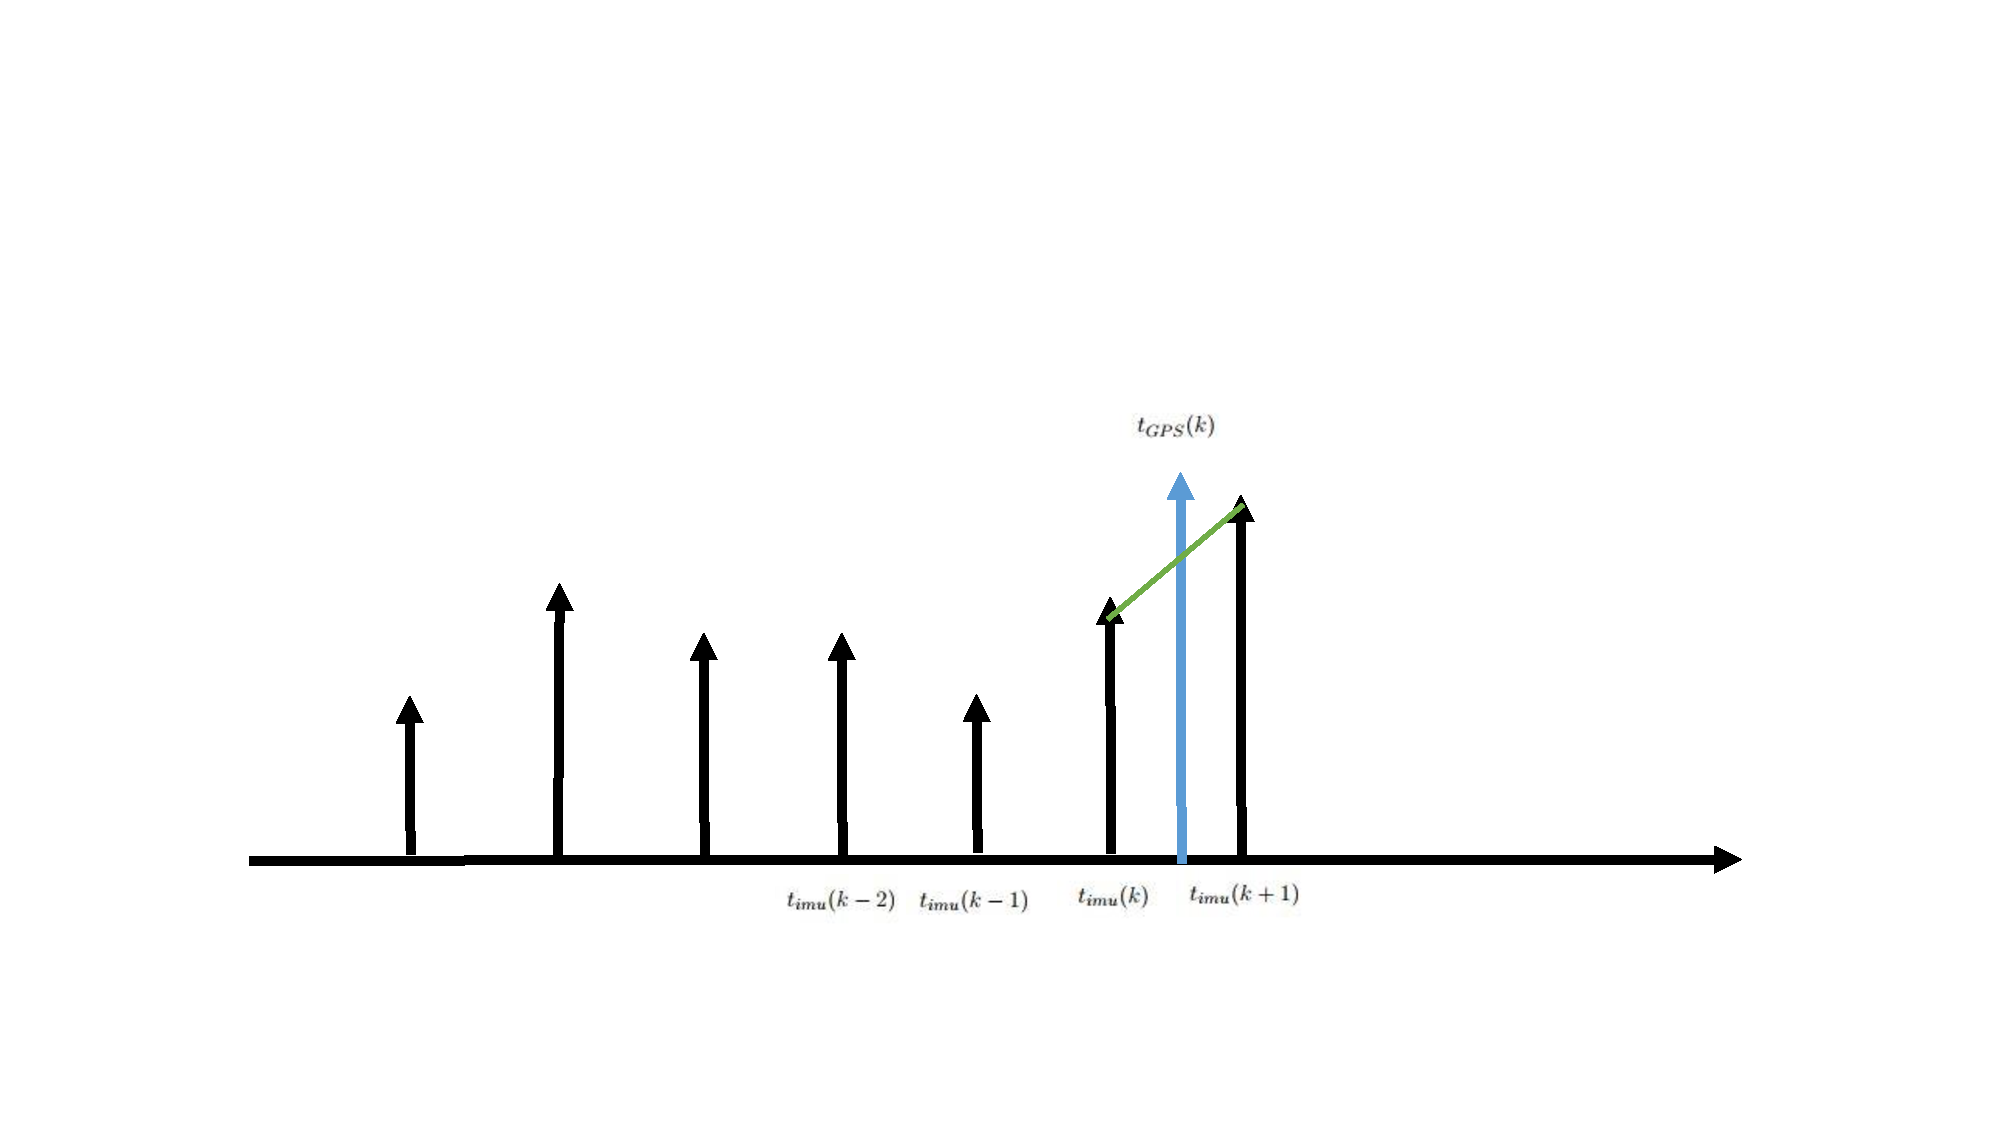
\includegraphics[width=0.8\textwidth]{Figures/linear.pdf}
\caption{Different update sequences \gls{imu} and \gls{gps}}
\label{Fig.different_update}
\end{figure}

The following linear interpolation equation is used for calculating the positions at $t_{GPS}(k)$
\begin{equation}
r_n(t_k(GPS) = r_n(t_{imu}(k)) + \frac{r_n(t_{imu}(k+1))-r_n(t_{imu}(k))}{t_{imu}(k+1)-t_{imu}(k)}(t_{GPS}(k)-t_{GPS}(k))
\end{equation}
 and the equations for the velocities 
 \begin{equation}
v_n(t_k(GPS) = v_n(t_{imu}(k)) + \frac{v_n(t_{imu}(k+1))-v_n(t_{imu}(k))}{t_{imu}(k+1)-t_{imu}(k)}(t_{GPS}(k)-t_{GPS}(k)).
\end{equation}
\subsection{Result}
The data provided by the Inertial Navigation System is working better than just using the raw \gls{gps} data, on some occasions. If the goal is to estimate the position, then it's better to use the \gls{ins} connected to a Kalman Filter, this can be seen in \autoref{Fig:result_kalman}. As seen, the Filtered data is inaccurate in the beginning but after some time converges to the true value, true value as in the case of wanted value, and at some points even catches the wanted value. In comparison to the raw \gls{gps} data, the \gls{ins} is a better estimator for the user's position.
\begin{figure}[H]
\centering
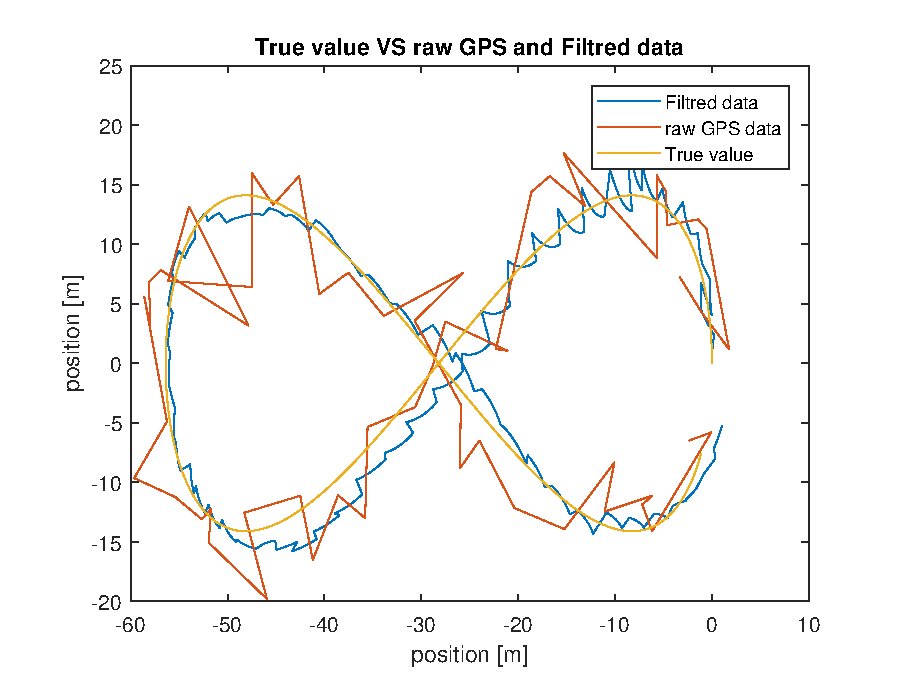
\includegraphics[width=0.5\textwidth]{result.eps}
\caption{True VS. Filtered and raw \gls{gps} data.}
\label{Fig:result_kalman}
\end{figure}



The Mean Squared Error, MSE for the position in XY plane, can be seen in \autoref{Fig:mse} for both \gls{ins} and raw \gls{gps} data we can see that the error is lower for the \gls{ins} data, in both cases. 
\begin{figure}[H]
\centering
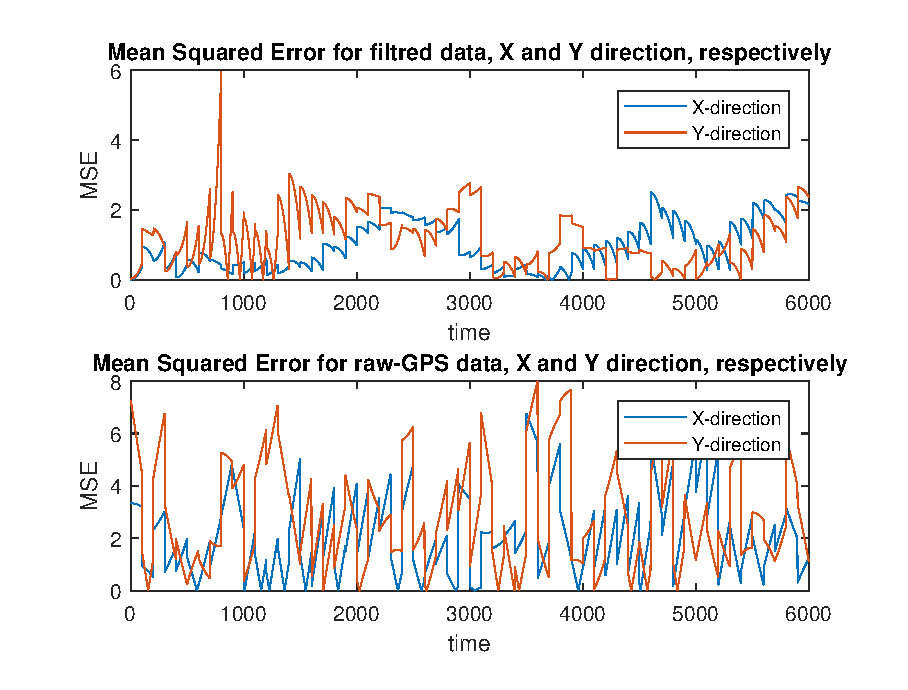
\includegraphics[width=0.5\textwidth]{mse.eps}
\caption{Mean Squared Error $XY$-plane separately.}
\label{Fig:mse}
\end{figure}

When estimating the height, i.e. $Z$-direction the result is poor for the \gls{ins}, the estimated value from the \gls{ins} is diverging from the true value, this can be seen in \autoref{Fig:Height}. In this case, the \gls{gps} data is more accurate. 
\begin{figure}[H]
\centering
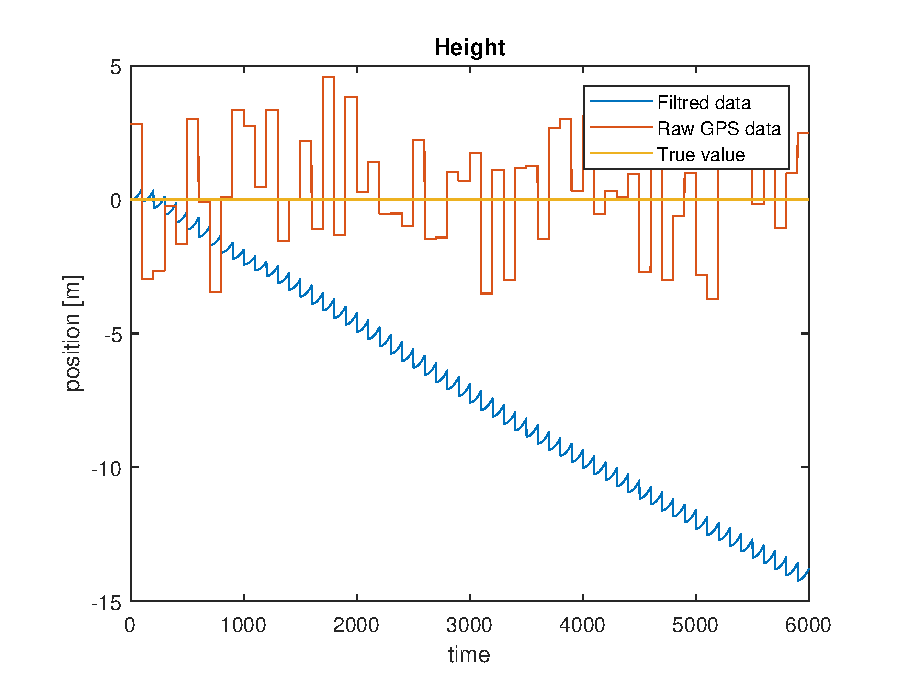
\includegraphics[width=0.5\textwidth]{Height.eps}
\caption{Height. True VS. Filtered and raw \gls{gps} data.}
\label{Fig:Height}
\end{figure}
The velocities in the $XY$ plane does not represent the true system in a good manner either this can be seen in \autoref{Fig:velocity}. In this case, the \gls{gps} data is more accurate as well.

\begin{figure}[H]
\centering
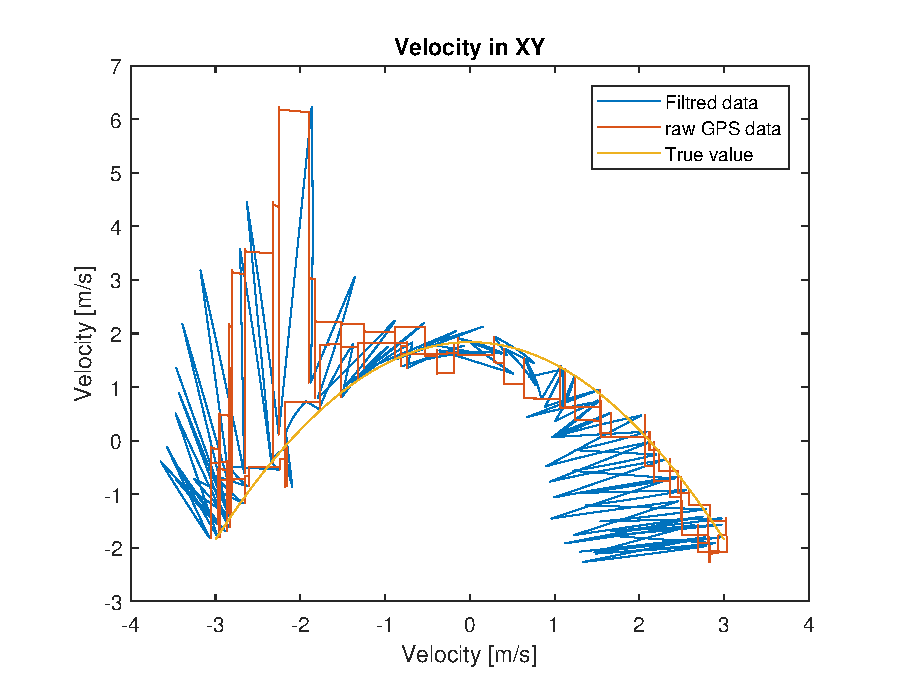
\includegraphics[width=0.5\textwidth]{velocity.eps}
\caption{The velocities in $XY$ plane.}
\label{Fig:velocity}
\end{figure}
\subsection{Discussion/Future Work}
Depending on what the user wants to measure, e.q. position in two dimensions, height or velocity, different sensors should be used. In the firts case, the \gls{ins} should be used in the case of the two latter the \gls{gps} should be used. \\

The Matlab code that exists, as right now, can read from the Nucleo Board using a serial read (assuming that the Nucleo Board uses the same firmware that was used by us), use stored data, (data created by our group) and also generate new data, with the \gls{imu} and \gls{gps} wanted characteristics. \\
Also, there is a static calibration program for the accelerometer. To see how the program works there exists a readme.txt file in the Matlab folder.\\

Implement a working real-time system for the sensor fusion between the \gls{gps} and \gls{ins}, there exits C-code for this already, but there is some serious bug/bugs which makes the error stored in $\hat{X}$ diverge exponentially. A serious attempt finding the problem was conducted and is narrowed down to a problem when calculating the Kalman Gain, $K_k$. Also, figure out why the height position diverges from the wanted value.\\

Improvements in the \gls{ins}/Kalman Filter implementation can be done as well, here are some thoughts that might be seen as guidelines/starting points to improve the system. \\
To obtain much more accurate information from the \gls{ins} one should consider more advanced techniques for calibrating the \gls{imu}. In this case, a static calibration technique was studied. This is done by keeping the \gls{imu} in a fixed position to observe the effect of gravity.
Consider implementing a more advanced technique, e.g. using this three-stage process.
\begin{itemize}
\item Coarse checking or evaluation using very simple test, such as a single stationary test on a bench, to establish the variance and standard deviation of the \gls{imu}, (gravity).
\item Static testing and studying the effects of natural phenomenon on the \gls{imu}.
\item Dynamic testing where the \gls{imu} is subjected to motions that should resemble the conditions out on the sea, e.g. constant waves hitting the sides of the boat. 
\end{itemize}
The purpose of this more advanced calibration technique is to determine the following parameters \cite{non-linear}
\begin{itemize}
\item scale factors
\item scale factor linearity
\item null bias error
\item axis alignment error, (might not be perfectly perpendicular)
\end{itemize}
Also, the dinghy's body may flex due to rough sea conditions, to solve this, implement one master \gls{ins} and one slave \gls{ins}, consider literature as Strap Down Inertial Navigation Technology, D.H. Titterton and J.L. Weston as a starting point for these different calibration methods. \newline 

A more advanced interpolation technique between \gls{imu} data and \gls{gps} data, here referencing to literature like Fundamentals of Scientific Computing, Bertil Gustafsson. E.g. Lagrange polynomial can be used to capture the true value better than using a linear interpolation.\newline


One should also try different types of control methods to see if one can achieve more accurate results or not, e.g. feed-forward method.\\
Weighted parameters if one believes the \gls{ins} more than the \gls{gps} or vice-versa, this question arises when e.g. the \gls{gps} is connected to many/few satellites or if the user is having a large/small velocity or sensor anomalies. 







\clearpage
\begin{thebibliography}{9}
\label{sec:ref}
\addcontentsline{toc}{section}{\nameref{sec:ref}}

% Reference to casing cad software missing
\bibitem{cad}
INSERT TEXT HERE
\bibitem{bqStudio}
Battery Management Studio (bqStudio) offers a full suite of robust tools to assist with the process of evaluating, designing with, configuring, testing, or otherwise utilizing TI Battery management products. \url{http://www.ti.com/tool/bqstudio}
\bibitem{stm32cubemx}
  \url{http://www.st.com/en/development-tools/stm32cubemx.html}
\bibitem{kicad}
  KiCad open source electronics design,
  \url{kicad-pcb.org/}
\bibitem{overprotection}
	Overvoltage and Reverce-voltage Protection in Automotive Systems,
	Application note 760, \emph{Maxim integrated}, Apr 02, 2002, 
	\url{https://www.maximintegrated.com/en/app-notes/index.mvp/id/760}
\bibitem{x-cube-ble1}
  \url{http://www.st.com/en/embedded-software/x-cube-ble1.html}
\bibitem{x-cube-mems1}
  \url{http://www.st.com/en/embedded-software/x-cube-mems1.html}
\bibitem{bluenrg-app}
  \url{http://play.google.com/store/apps/details?id=com.st.blunrg}
\bibitem{x-nucleo-idb05a1}
  \url{http://www.st.com/en/ecosystems/x-nucleo-idb05a1.html}
\bibitem{x-nucleo-iks01a2}
  \url{http://www.st.com/en/ecosystems/x-nucleo-iks01a2.html}
\bibitem{madgwick}
  \url{http://x-io.co.uk/open-source-imu-and-ahrs-algorithms}
\bibitem{madgwick-report}
  \url{http://x-io.co.uk/res/doc/madgwick_internal_report.pdf}
\bibitem{gps}
  \url{http://update.maestro-wireless.com/GNSS/A2235-H/Maestro_GPS_Evaluation_Kit_EVA2235_H_User_Manual_V01.pdf}
\bibitem{libnmea}
  \url{http://github.com/jacketizer/libnmea}
\bibitem{x-cube-53l0a}
  \url{http://www.st.com/content/st_com/en/products/ecosystems/stm32-open-development-environment/stm32-nucleo-expansion-boards/stm32-ode-sense-hw/x-nucleo-53l0a1.html}
\bibitem{android-service}
  \url{https://developer.android.com/reference/android/app/Service.html}
\bibitem{lat-long-calc}
  \url{https://www.movable-type.co.uk/scripts/latlong.html}
\bibitem{lm1117}
	KiCad library entry for voltage regulator component lm1117 by \emph{ObKo}, 2012  
  \url{https://github.com/ObKo/kicad-libraries/blob/master/libraries/lm1117.lib}
\bibitem{llc}
	Bi-directional Logic Level Converter, \emph{Sparkfun}, Aug 4, 1997,
	\url{https://cdn.sparkfun.com/tutorialimages/BD-LogicLevelConverter/an97055.pdf}
\bibitem{ftdi}
	KiCad library entry for USBtoSerial component FT232RL by \emph{jbaker0428}, Oct 3, 2010
	\url{https://github.com/jbaker0428/Kicad-Libraries/blob/master/library/ftdi.lib}
\bibitem{rhumb-line}
  \url{https://en.wikipedia.org/wiki/Rhumb_line}
\bibitem{equirectangular}
  \url{https://en.wikipedia.org/wiki/Equirectangular_projection}
\bibitem{haversine}
  \url{https://en.wikipedia.org/wiki/Haversine_formula}
\bibitem{sailing}
  \url{https://en.wikipedia.org/wiki/Sailing}
\bibitem{sail-force}
  \url{http://newt.phys.unsw.edu.au/~jw/sailing.html}
\bibitem{volvo}
  \url{https://sv.wikipedia.org/wiki/Volvo_Amazon}
\bibitem{png}
  \url{https://sv.wikipedia.org/wiki/PNG}
\bibitem{activity}
  \url{https://developer.android.com/reference/android/app/Activity.html}
\bibitem{uml}
  \url{https://en.wikipedia.org/wiki/Unified_Modeling_Language}
\bibitem{gl}
  \url{https://developer.android.com/reference/android/opengl/GLSurfaceView.html}
\bibitem{texttospeech}
  \url{https://developer.android.com/reference/android/speech/tts/TextToSpeech.html}
\bibitem{utter}
  \url{https://developer.android.com/reference/android/speech/tts/UtteranceProgressListener.html}
\bibitem{gmaps}
  \url{https://developers.google.com/maps/}

\bibitem{animal} 
D.L. Hall and J. Llinas. An introduction to multisensor data fusion. 
\textit{Proceedings of the}. IEEE, 85(1):6 –23, jan 1997

\bibitem{boken} 
B.R. Grover H. Patrick. Introduction to random signals and applied Kalman filtering. 1997
\textit{BOKEN}. 

\bibitem{SNAME} 
Society of Naval Architects and Marine Engineers (SNAME), "Principles of Naval Architecture", 1989, Vol. III,
\textit{SNAME}. 

 
\bibitem{nonlinear} 
Dr. Oliver Nelles
\\\texttt{nonlinear system identification.}

\bibitem{kf eff}
Duygun, M., Kutlu, L. \& Sickles, R.C. J Prod Anal (2016) 46: 155. \url{https://doi.org/10.1007/s11123-016-0477-z}
\bibitem{non-linear}
Noureldin ., Karamat T.B., Georgy J. (2013)\texttt{ Basic Navigational Mathematics, Reference Frames and the Earth’s Geometry. In: Fundamentals of Inertial Navigation, Satellite-based Positioning and their Integration.} Springer, Berlin, Heidelberg
\bibitem{cccv}
	Power Guy, \emph{Constant Current Constant voltage}, May 26, 2016, San Diego, USA,
  \url{https://www.us.tdk-lambda.com/media/292143/tdk-lambda-blog-052616.pdf}
\bibitem{UoC}
  \url{https://edg.uchicago.edu/tutorials/load_cell/}
\bibitem{animal}
D.L. Hall and J. Llinas. An introduction to multisensor data fusion. 
\textit{Proceedings of
the}. IEEE, 85(1):6 –23, jan 1997

\bibitem{signal_process}
Probability and Random Processes with Applications to Signal Processing, 4/E (2012). 
Henry Stark, John W Woods. Pearson Higher Education. 

\bibitem{Discrete_kalman}
	Donald E. Catlin, \emph{Estimation, Control, and the Discrete Kalman Filter}, 1989
\bibitem{pertubation}
  \url{https://en.wikipedia.org/wiki/Perturbation_theory}

\bibitem{book}%[p.26-27]
Weicker, P. (2014). \emph{A Systems Approach to Lithium-ion Battery Management}, Boston, Artech House. 

%\bibitem{book}[p.111]
%Weicker, P. (2014). A Systems Approach to Lithium-ion Battery Management. (pp.111). Boston: Artech House. 

%\bibitem{book}[p.111-112]
%Weicker, P. (2014). A Systems Approach to Lithium-ion Battery Management. (pp.111-112). Boston: Artech House.

%\bibitem{book}[p.183-185]
%Weicker, P. (2014). A Systems Approach to Lithium-ion Battery Management. (pp.183-185). Boston: Artech House.

%\bibitem{book}[p.35-38]
%Weicker, P. (2014). A Systems Approach to Lithium-ion Battery Management. (pp.35-38). Boston: Artech House.

\bibitem{webpage}
  \url{http://www.lygte-info.dk/info/battery%20protection%20UK.html}
(pp. [Page number starts]-[ends]).

\end{thebibliography}


\end{document}
